\chapter{Cardea}\label{sec-cardea}

\section{System Design}
Recalling related works in Chapter 2, what motivates the design of Cardea are the following:

\begin{itemize}
\item People's privacy concerns are dependent on context. Although in certain circumstances locations are strong hints of possible privacy intrusion, generally what individuals are doing and with whom are more essential and crucial factors that directly relate to privacy.
\item People's privacy preferences vary from each other, thus they should be able to express their personal privacy preferences.
\item People's privacy preferences may change from time to time, therefore they need a way to change such preferences easily.
\end{itemize}

To achieve these objectives, we propose following solution:
\begin{itemize}
  \item We combine GPS location, grouped scene categories (Table~\ref{tbl-scenecate}) and accompanied persons as context that can better represent people's privacy concerns than previous methods. As a result we are able to provide more general as well as finer granularity privacy preference settings for users.
\item We use cloud server to host individualized privacy preferences, and user's preference is bound with his facial features. In this way his raw visual information stays locally, preventing the case of visual privacy leakage from hacked servers.
\item Other than a simple interface provided to users to update their privacy preferences, hand gestures like \vcenteredinclude{figure/ch4-yesgesticon.png} and \vcenteredinclude{figure/ch4-nogesticon.png} can be used by user to actively speak out about his preference in the capturing moment, enriching the interaction and adding more flexibilities.
\end{itemize}
As introduced in chapter 3, breakthroughs made by deep learning community in many computer vision problems such as image classification, face recognition and object detection have guided the proposed solution and shed lights on its practicability. More specifically, given a captured image, Cardea will leverage powerful convolutional neural networks for the recognition of scene context, registered users and gestures. Cardea's design is given in Fig~\ref{fig:ch4-cardeadesign}, it is composed of the client applications and cloud server. It works based on data exchange and collaborative computing involving both client and cloud sides. The major components and interactions include:
\begin{figure}[!htbp]
    \centering
    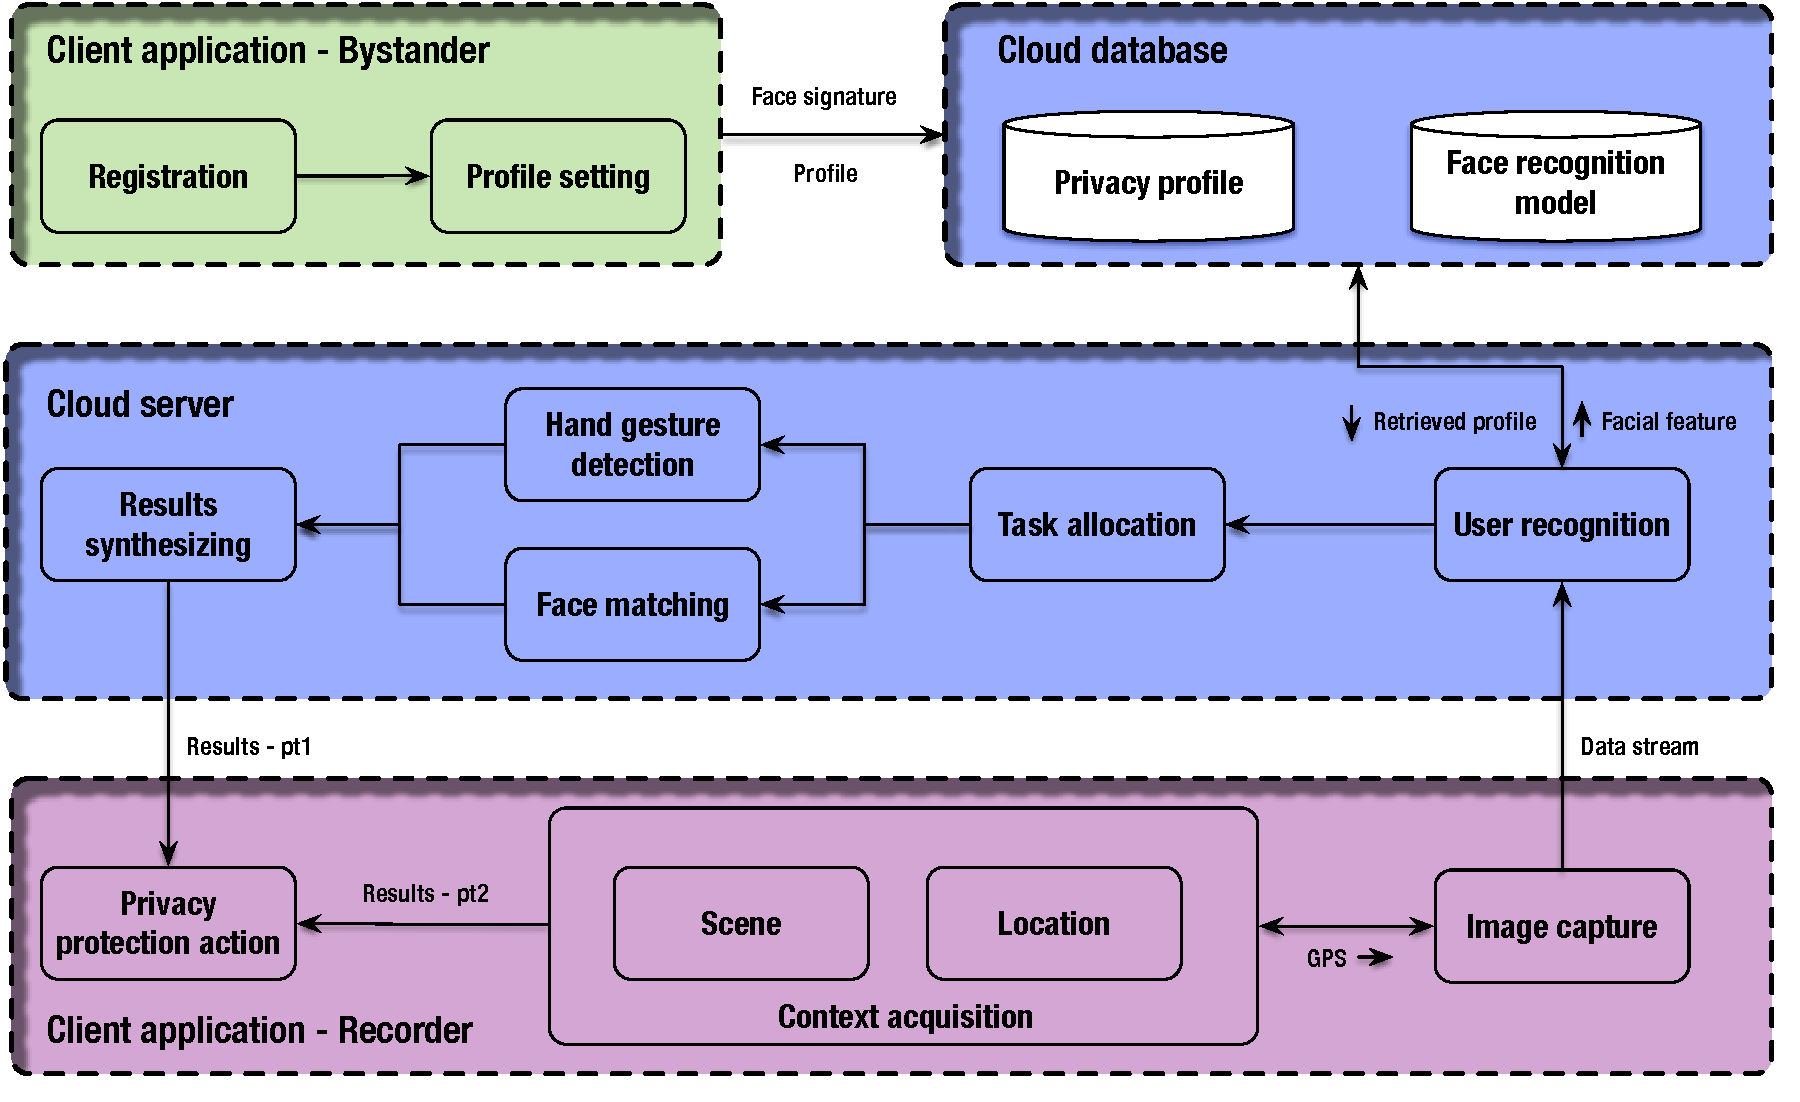
\includegraphics[width=1.0\textwidth]{figure/ch4-cardeadesign.pdf}
    \caption{System design of Cardea.}
    \label{fig:ch4-cardeadesign}
\end{figure}

\begin{description}[leftmargin=0cm]
  \item[{\bfseries Bystander client application:}] A bystander can use this application to register as Cardea user and define his privacy profile. It will capture a number of face images (about 50--60 images) and extract facial features from these images as his unique face signature. After setting up the context dependant privacy preference, his facial signature and preference will be sent to cloud server for registration and updating of face recognition model.
  \item[{\bfseries Recorder client application:}] A recorder can use this application to take images that will automatically perform privacy protection actions in compliance with all Cardea users' privacy preferences. Given a captured image, it first detects all the faces and extracts the corresponding facial features locally on device, then the features and the captured image (compressed and with all detected faces blurred) are sent to the server for face and gesture recognitions. GPS coordinate is also sent to server in this step to be compared with recognized users' location settings. During the time waiting for response from cloud, it performs scene group prediction task. Finally, predicted scene group and intermediate decision result received from server are combined to decide the actual protection action which will be enforced on the raw captured image.
  \item[{\bfseries Cloud server:}] The cloud server plays two roles: \ding{182} When receiving requests from Bystander applications, it will store/update users' profiles, and training/updating system's face recognition model automatically; \ding{183} When receiving requests from Recorder applications, it will initiate face and gesture recognition tasks, as well as partial decision making based on recognition results, and send these intermediate decision results to client for the final step of decision making.
\end{description}

% Implementations of each module, how Cardea allocates tasks between mobile and cloud, integration, usage and performance evaluation of the whole system are discussed throughly in following sections.

Implementations and evaluation of each module, how Cardea allocates tasks between mobile and cloud, integration and user interactions are discussed in following sections.

\begin{table}[tb]
\centering
\caption{Scene categories.}
\label{tbl-scenecate}
\begin{tabular}{ll}
\toprule
Scene Group    & Scene Category                                       \\ \midrule
Eating         & bistro/indoor, bistro/outdoor, cafeteria, coffee\_shop, \\
               & diner/outdoor, dining\_hall, dining\_room, fastfood\_restaurant, food\_court, \\
               & restaurant, restaurant\_patio, sushi\_bar            \\ \midrule
Entertainment  & bar, discotheque, pub/indoor                         \\ \midrule
Shopping       & bazaar/indoor, bazaar/outdoor, clothing\_store, general\_store/indoor, \\
               & jewelry\_shop, shoe\_shop, shopping\_mall/indoor, supermarket  \\ \midrule
Work           & conference\_center, conference\_room, cubicle/office, library/indoor, office, \\
               & office\_cubicles, reading\_room                      \\ \midrule
Public         & park, street                                         \\ \midrule
Mobility       & airplane\_cabin, airport\_terminal, bus\_interior, bus\_station/indoor, \\
               & subway\_station/platform, train\_interior, train\_station/platform \\ \midrule
Exhibition     & art\_gallery, museum/indoor                          \\ \midrule
Religion       & cathedral/indoor, cathedral/outdoor, church/indoor, church/outdoor, mosque/outdoor, \\
               & pulpit, temple/east\_asia, temple/south\_asia        \\ \midrule
Illness        & hospital, hospital\_room, nursing\_home                \\ \midrule
Nudity         & bathroom, beach, jacuzzi/indoor, sauna, shower, \\
               & swimming\_pool/indoor, swimming\_pool/outdoor        \\ \bottomrule
\end{tabular}
\end{table}

\section{Model Training}

\subsection{Scene Classification}

\subsubsection{Data Preparing and Preprocessing}

For scene classification, we use pre-trained model of Places2 dataset provided by~\cite{links:places2mit}. In the time Cardea project was conducted, Places2 dataset provided by the authors contained 401 categories with more than 8 million training images, and the pre-trained model was based on AlexNet structure~\cite{krizhevsky2012imagenet}. By the time this thesis is writing, the dataset is deprecated and the new Places2 dataset contains 365 categories. And the authors provide more pre-trained models based on different network structures~\cite{links:places2pre}.

\begin{figure}[!htbp]
    \centering
    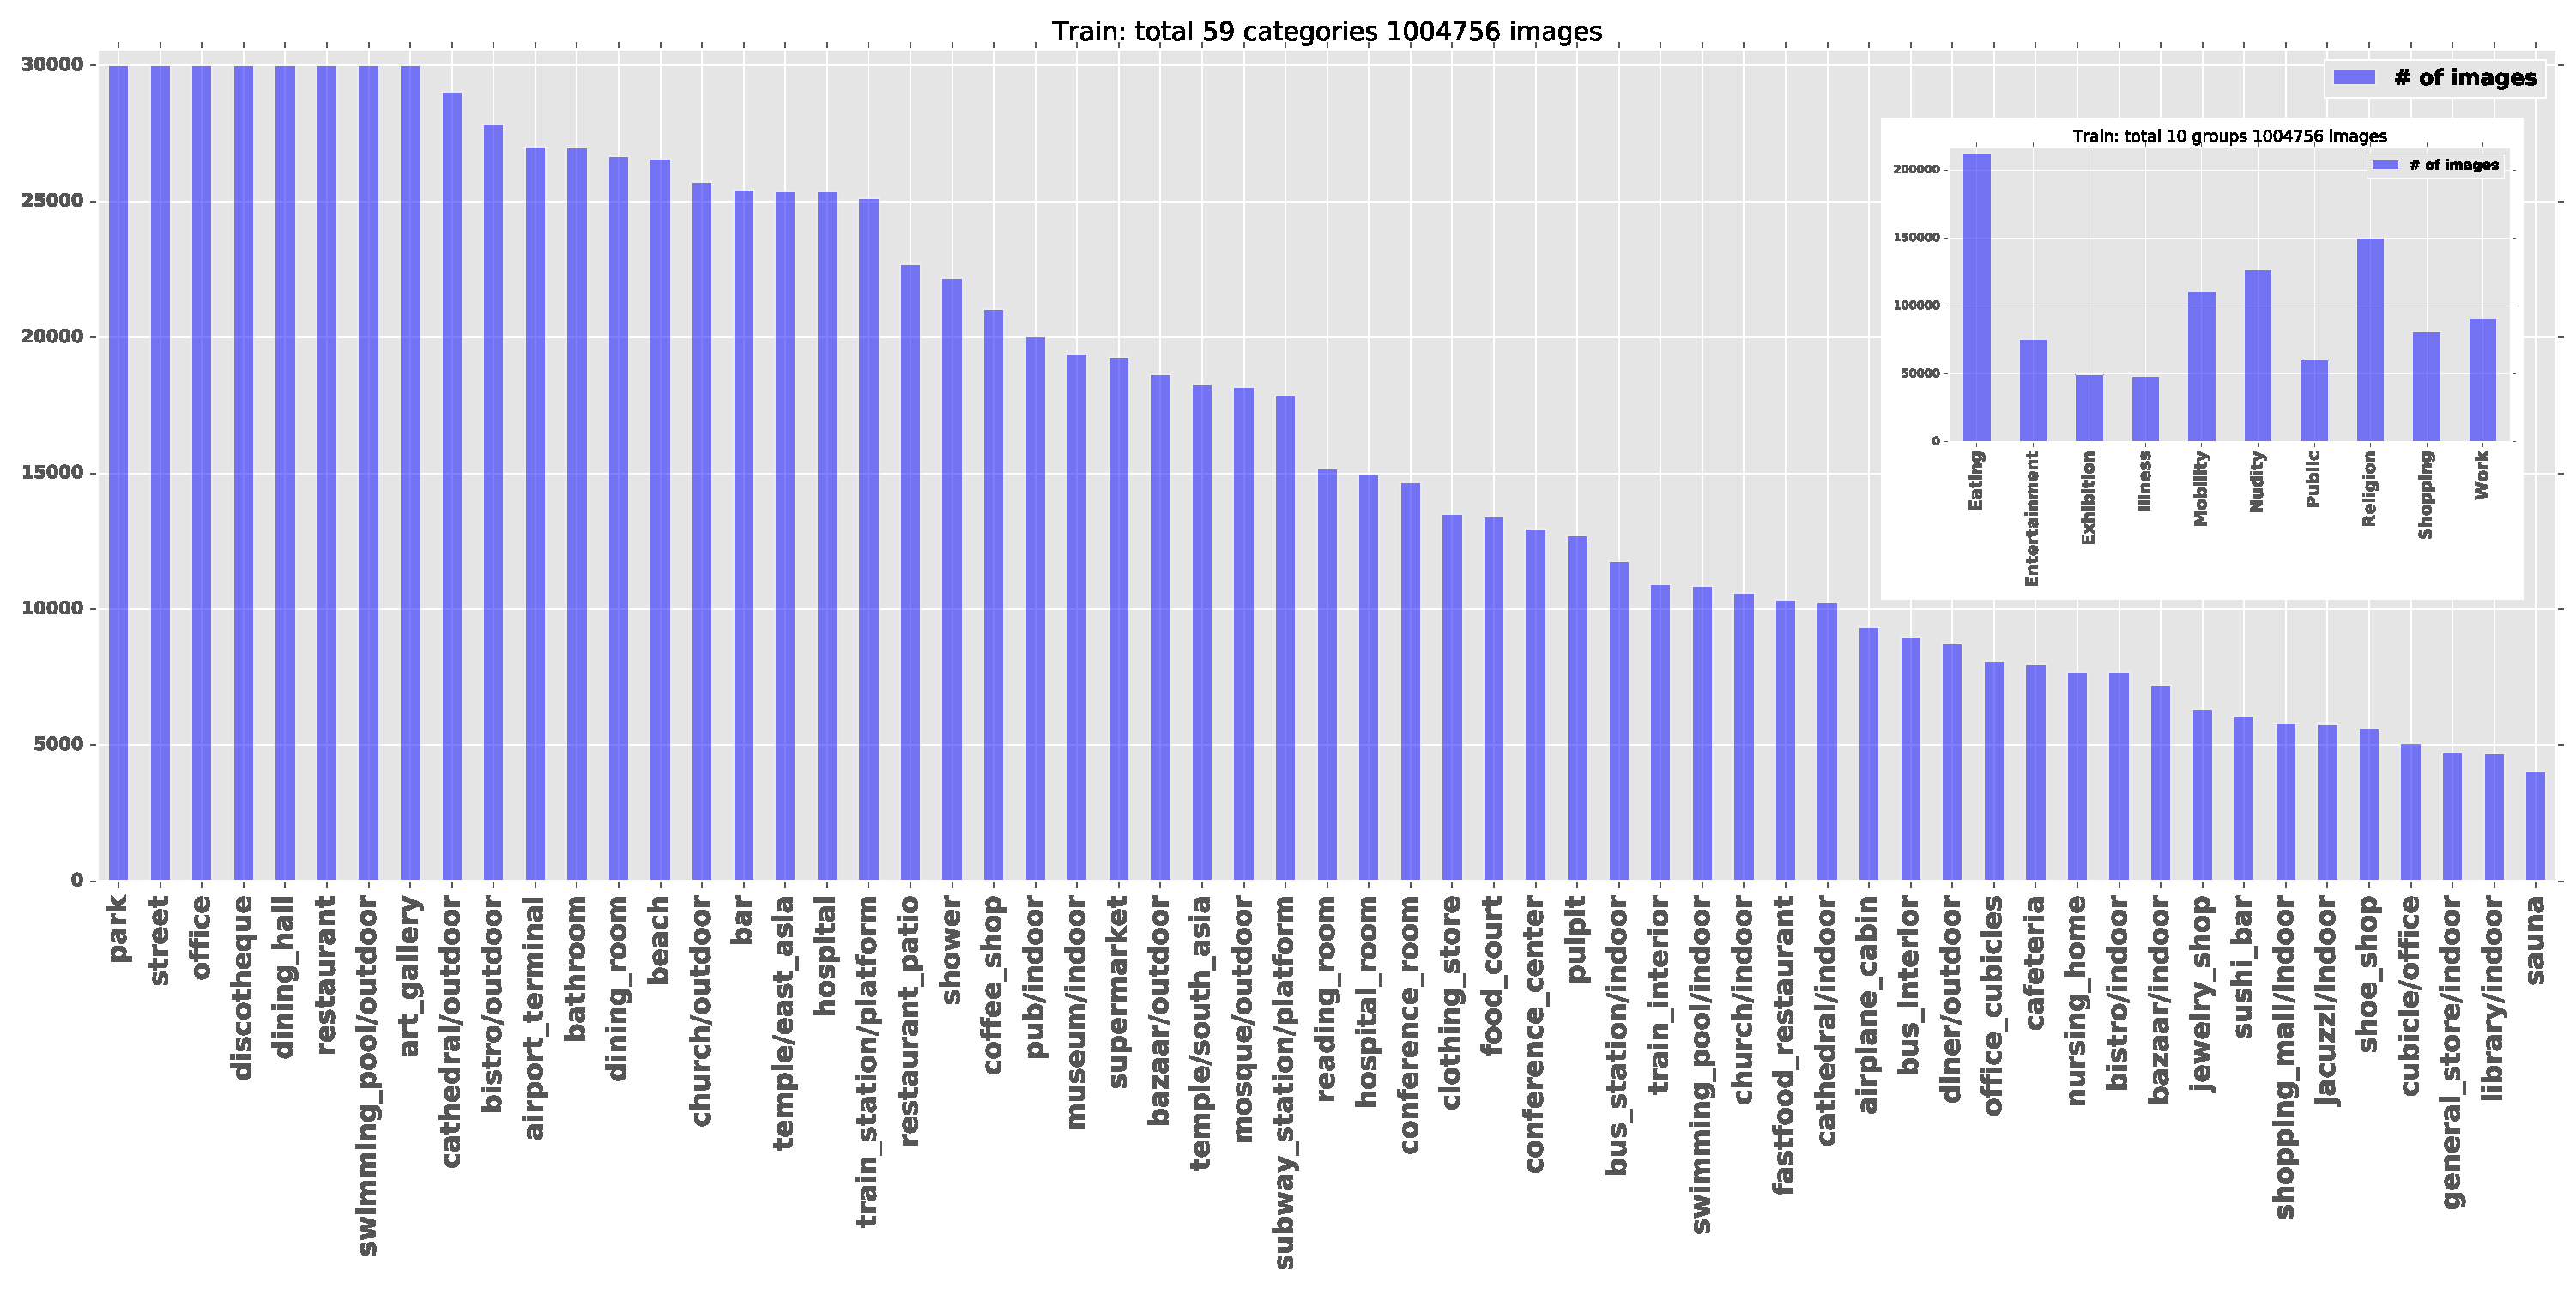
\includegraphics[width=1.0\textwidth]{figure/ch4-numdist.pdf}
    \caption{Number of images for each category and each group (inset).}
    \label{fig:ch4-scenenumdist}
\end{figure}

Note that in the dataset we used, there is a non-uniform distribution of images per category for training, ranging from 4,000 to 30,000, mimicking a natural frequency of occurrence of the scene. Among the 401 categories, we choose 59 scene categories that are close to daily life and in such scenes people may have privacy concern. In total this subset composed of 1 million training images and 2950 validation images (50 validation images for each category). We also group these 59 scene categories into 10 groups based on contextual similarity as shown in Table~\ref{tbl-scenecate}, such that people have similar reasons for privacy concerns in scenes that are in the same group (e.g. people don't want to be captured in bathroom and beach is both because of nudity concerns). The distribution of training images among categories and groups is shown in Fig~\ref{fig:ch4-scenenumdist}.

\subsubsection{Training Procedures}
The training step is a standard fine-tuning process, which is extensively used in transfer learning~\cite{sharif2014cnn,yosinski2014transferable}:

\begin{itemize}
\item[\ding{182}] Using pre-trained model as feature extractor, we extract the features at \emph{fc7} layer for images belonging to the 59 picked categories. Other than shuffling the features, we also augment the features such that all categories have same amount of features. Though the natural frequencies of occurrence are obviously different among different scenes, we argue that for the purpose of privacy protection, all the scene categories should be equally important, thus categories imbalance is not what we favored. The augmentation step can be implemented using weighted loss layer, but we take simple way of bootstrapping features for categories with less images. After this step, all features are cached and stored in lmdb format.
\item[\ding{183}] Train a softmax classifier of the 59 categories using the extracted features. We choose to train a classifier for categories and then add up the output probabilities to predict the group, rather than directly train a group classifier, is because category classifier tells more about the image, and our desired property is equal weights among scene categories rather than groups.
\item[\ding{184}] Both feature extraction and classifier training are implemented using Caffe library~\cite{links:caffelib,jia2014caffe}. In this step we merge the feature extraction part of pre-trained model and the softmax classifier into a single model by copying weights. Now Caffe has the option of specifying layers with fixed weights, thus simplifying the fine-tuning and deployment process.
\end{itemize}

Other than improving the validation accuracy from 0.56 to 0.57, shuffling also makes training converges faster. With augmentation to relieve category imbalance issue, the classifier can finally achieve 0.600 validation accuracy on the 59 categories. There is no other benchmarking result specifically on the subset we choose, but recent benchmark gives 53\%-56\% validation accuracy on the new Places2 dataset with 365 categories~\cite{links:places2pre}, suggesting our model is competitive. The higher validation accuracy of our model is due to the smaller scale of classification problem we are dealing with.

\subsubsection{Prediction}

\begin{figure}[!t]
    \centering
    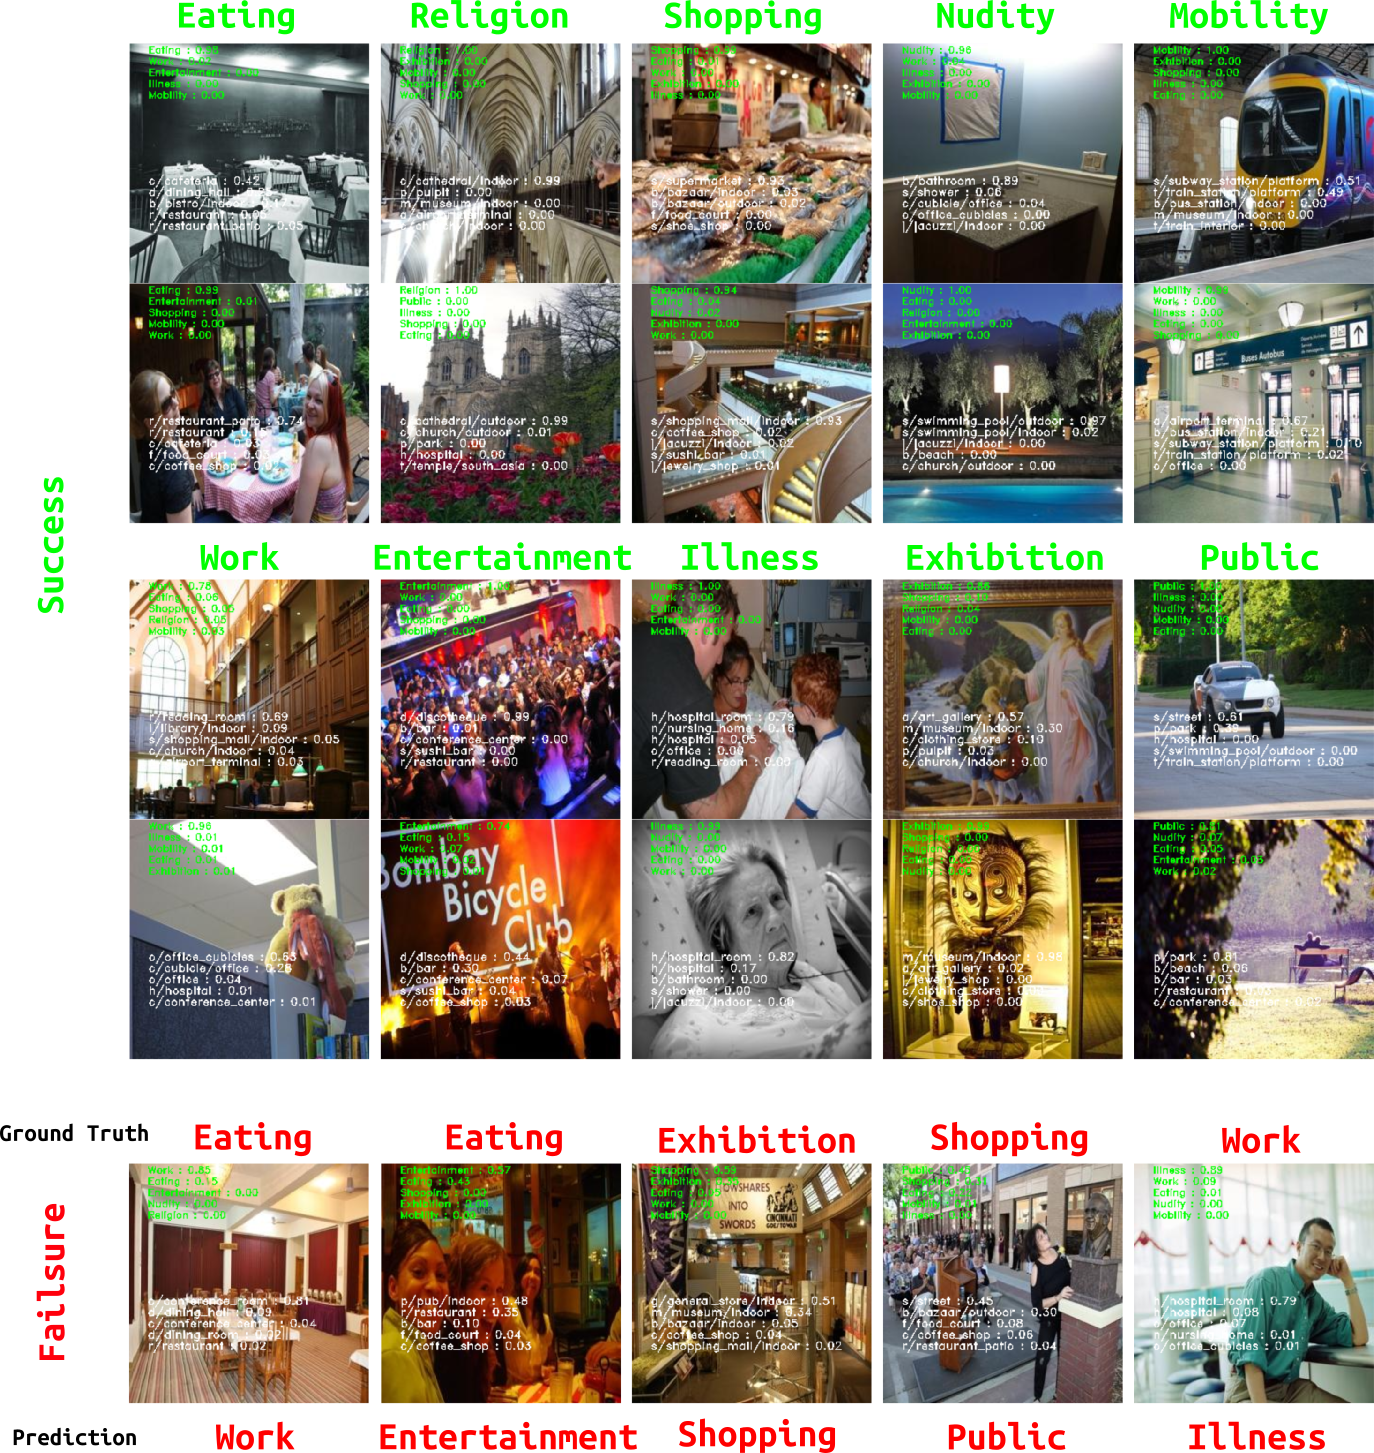
\includegraphics[width=\textwidth]{figure/ch4-scnpredictemp.png}
    \caption{Scene classification prediction example. Top5 groups (green) and categories (white) are shown with their probabilities.}
    \label{fig:ch4-scnpredictemp}
\end{figure}

For prediction, we get probability of a group by summing up the probabilities of all categories belonging to this group, and output the most probable group as prediction of an image. Our model's group prediction accuracy for the validation set is 82.8\%. Fig~\ref{fig:ch4-scnpredictemp} shows some prediction examples. As seen from the examples, given an image, the predicted category probabilities are usually distributed to few categories within same group, thus group prediction is resilient to perturbation coming from category prediction. The way we group categories can be seemed as a hard-coded clustering step, which makes prediction more robust to noise. The failure cases are mostly due to natural context ambiguity from a image (e.g. image with object in focus, therefore not enough hints for scene inference). Labeling the 342 non selected categories as an extra group will amplify the ambiguity issue, as doing so will distribute probabilities to the extra group and lead to wrong prediction, even for images with less ambiguity. In other words, a 59 way classifier leads to higher recall for selected scenes and grouping leads to higher accuracy. This is also reflected in confusion matrices shown in Fig~\ref{fig:ch4-scnconfumat}, category confusion matrix shows some clustering structure which is in accordance with the groups we manually assigned. However, only using top 1 category for prediction sacrifices prediction accuracy, which can be avoided by grouping as shown in group confusion matrix.

\begin{figure}[!htbp]
    \makebox[\textwidth]{
        \centering
        \raisebox{-0.5\height}{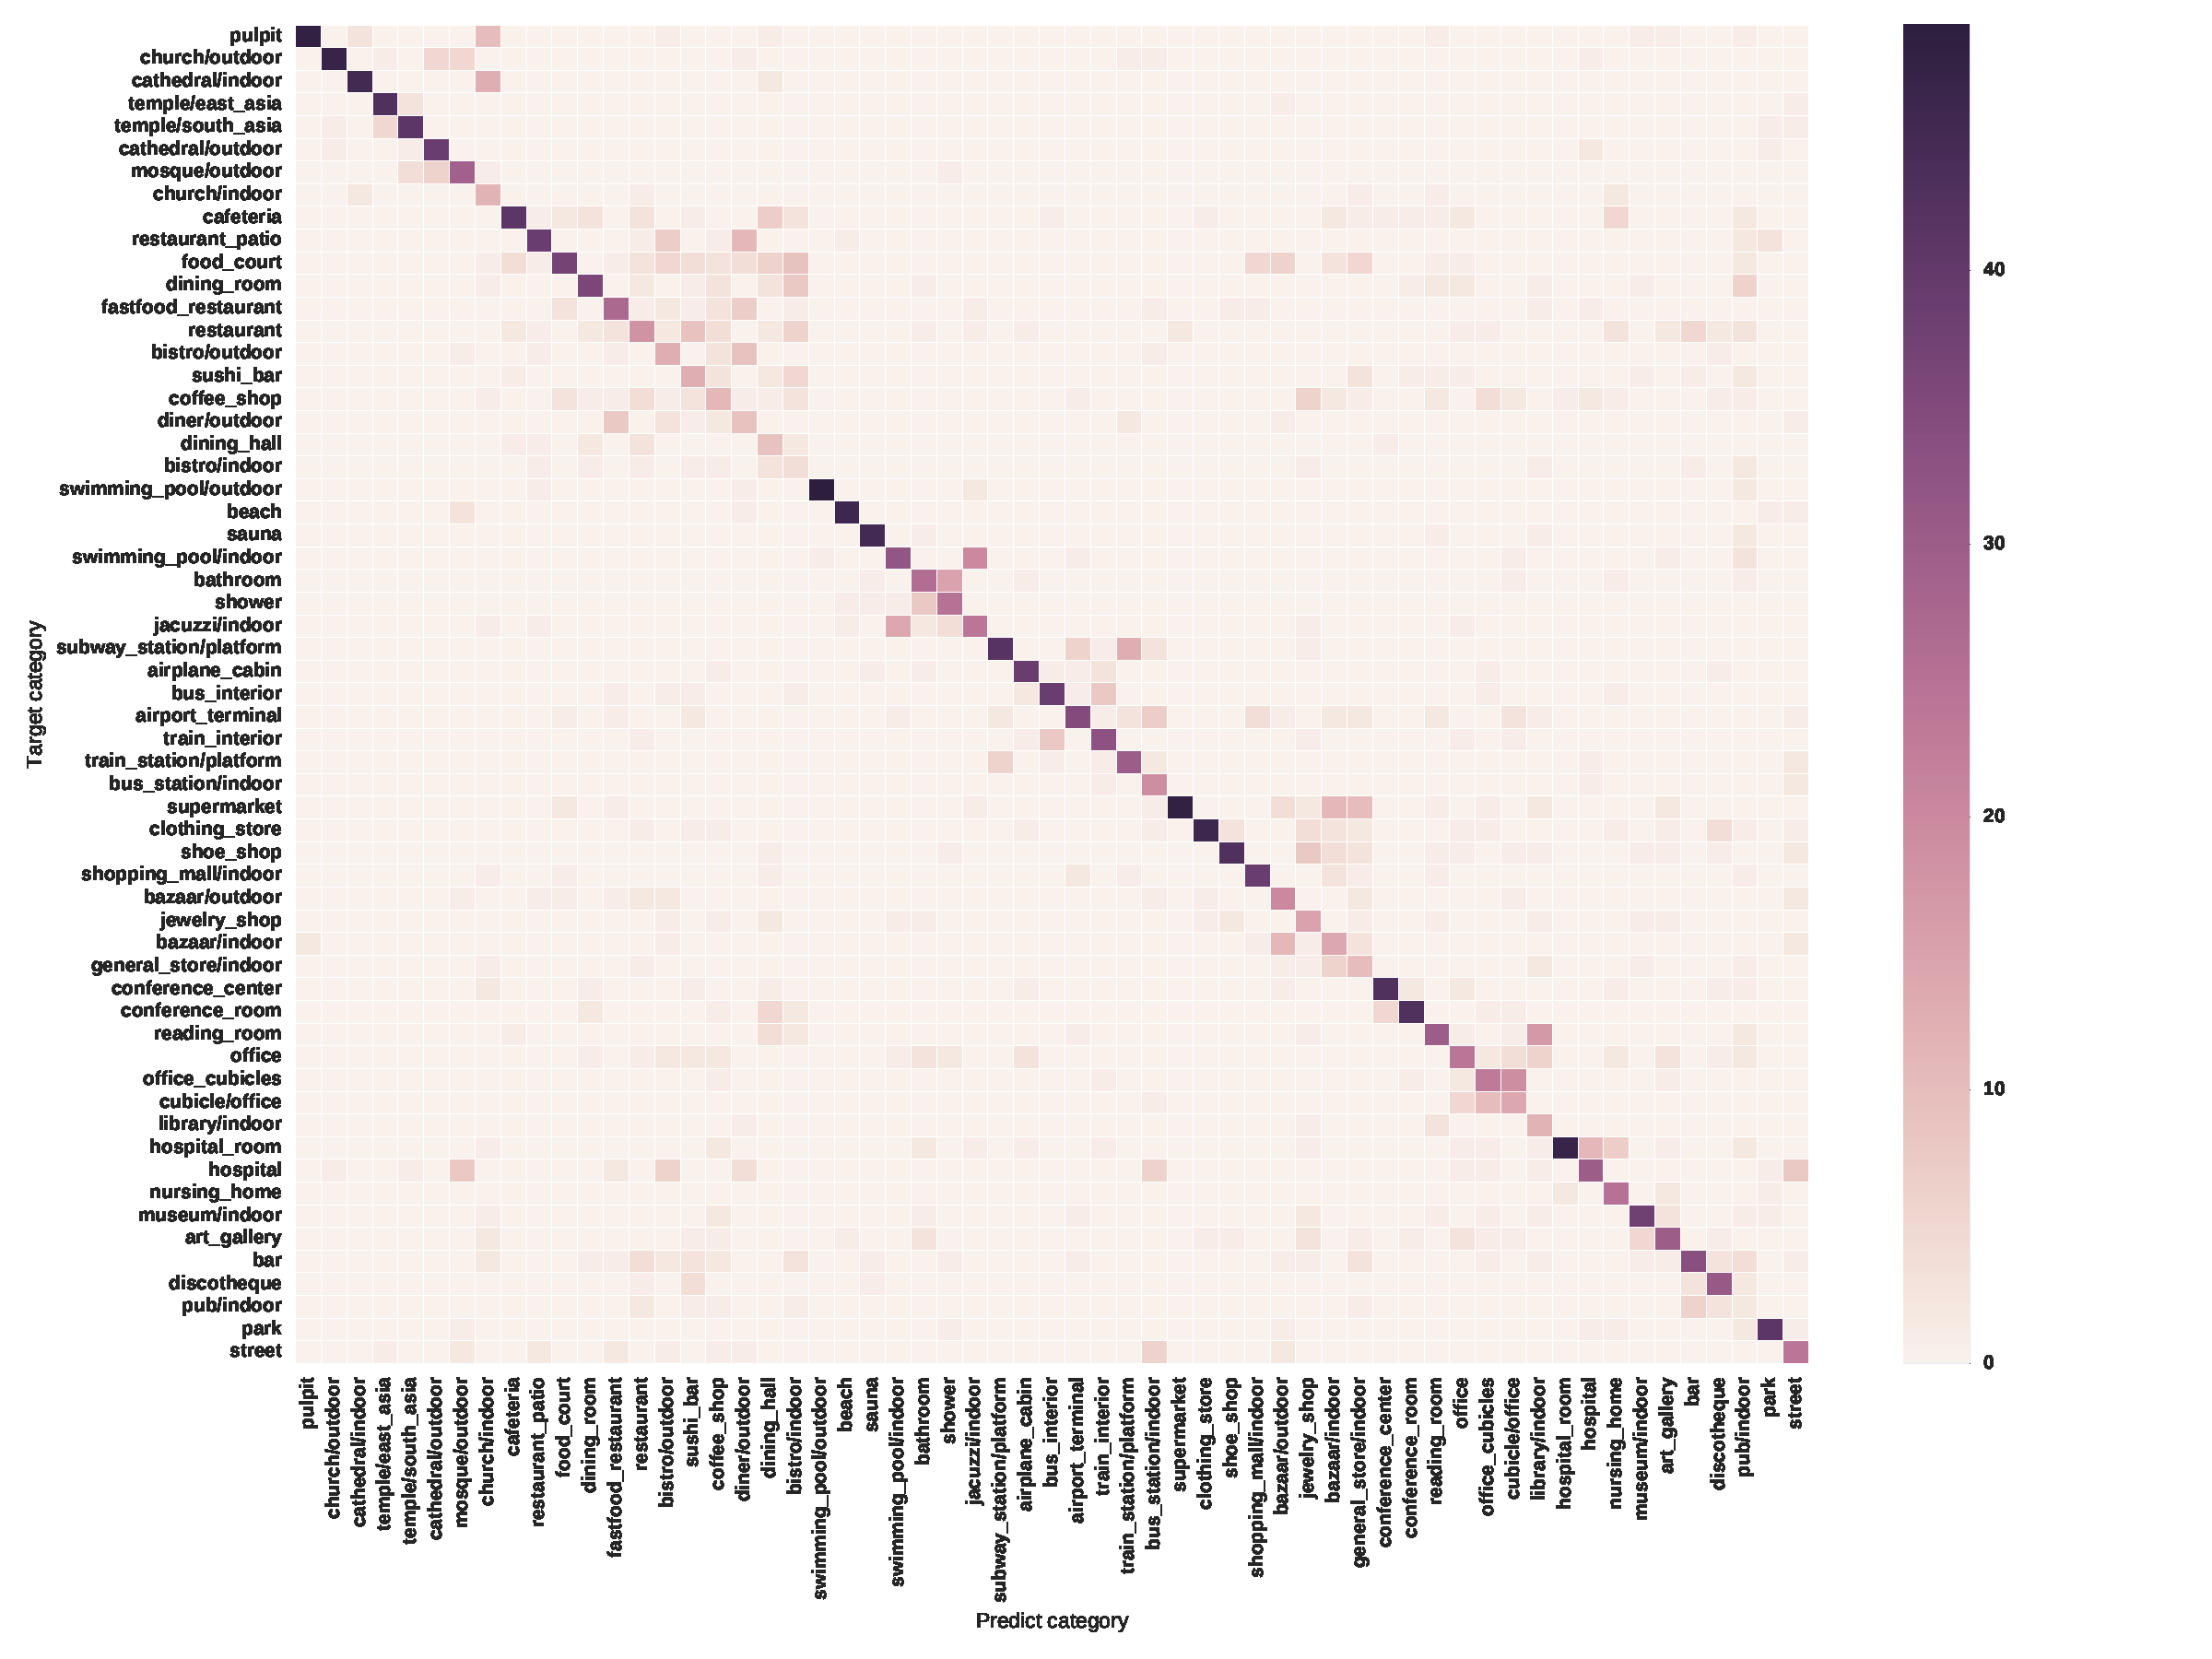
\includegraphics[width=0.7\textwidth]{figure/ch4-scnCateConfu.pdf}}
        \hspace{-1cm}%
        \raisebox{-0.5\height}{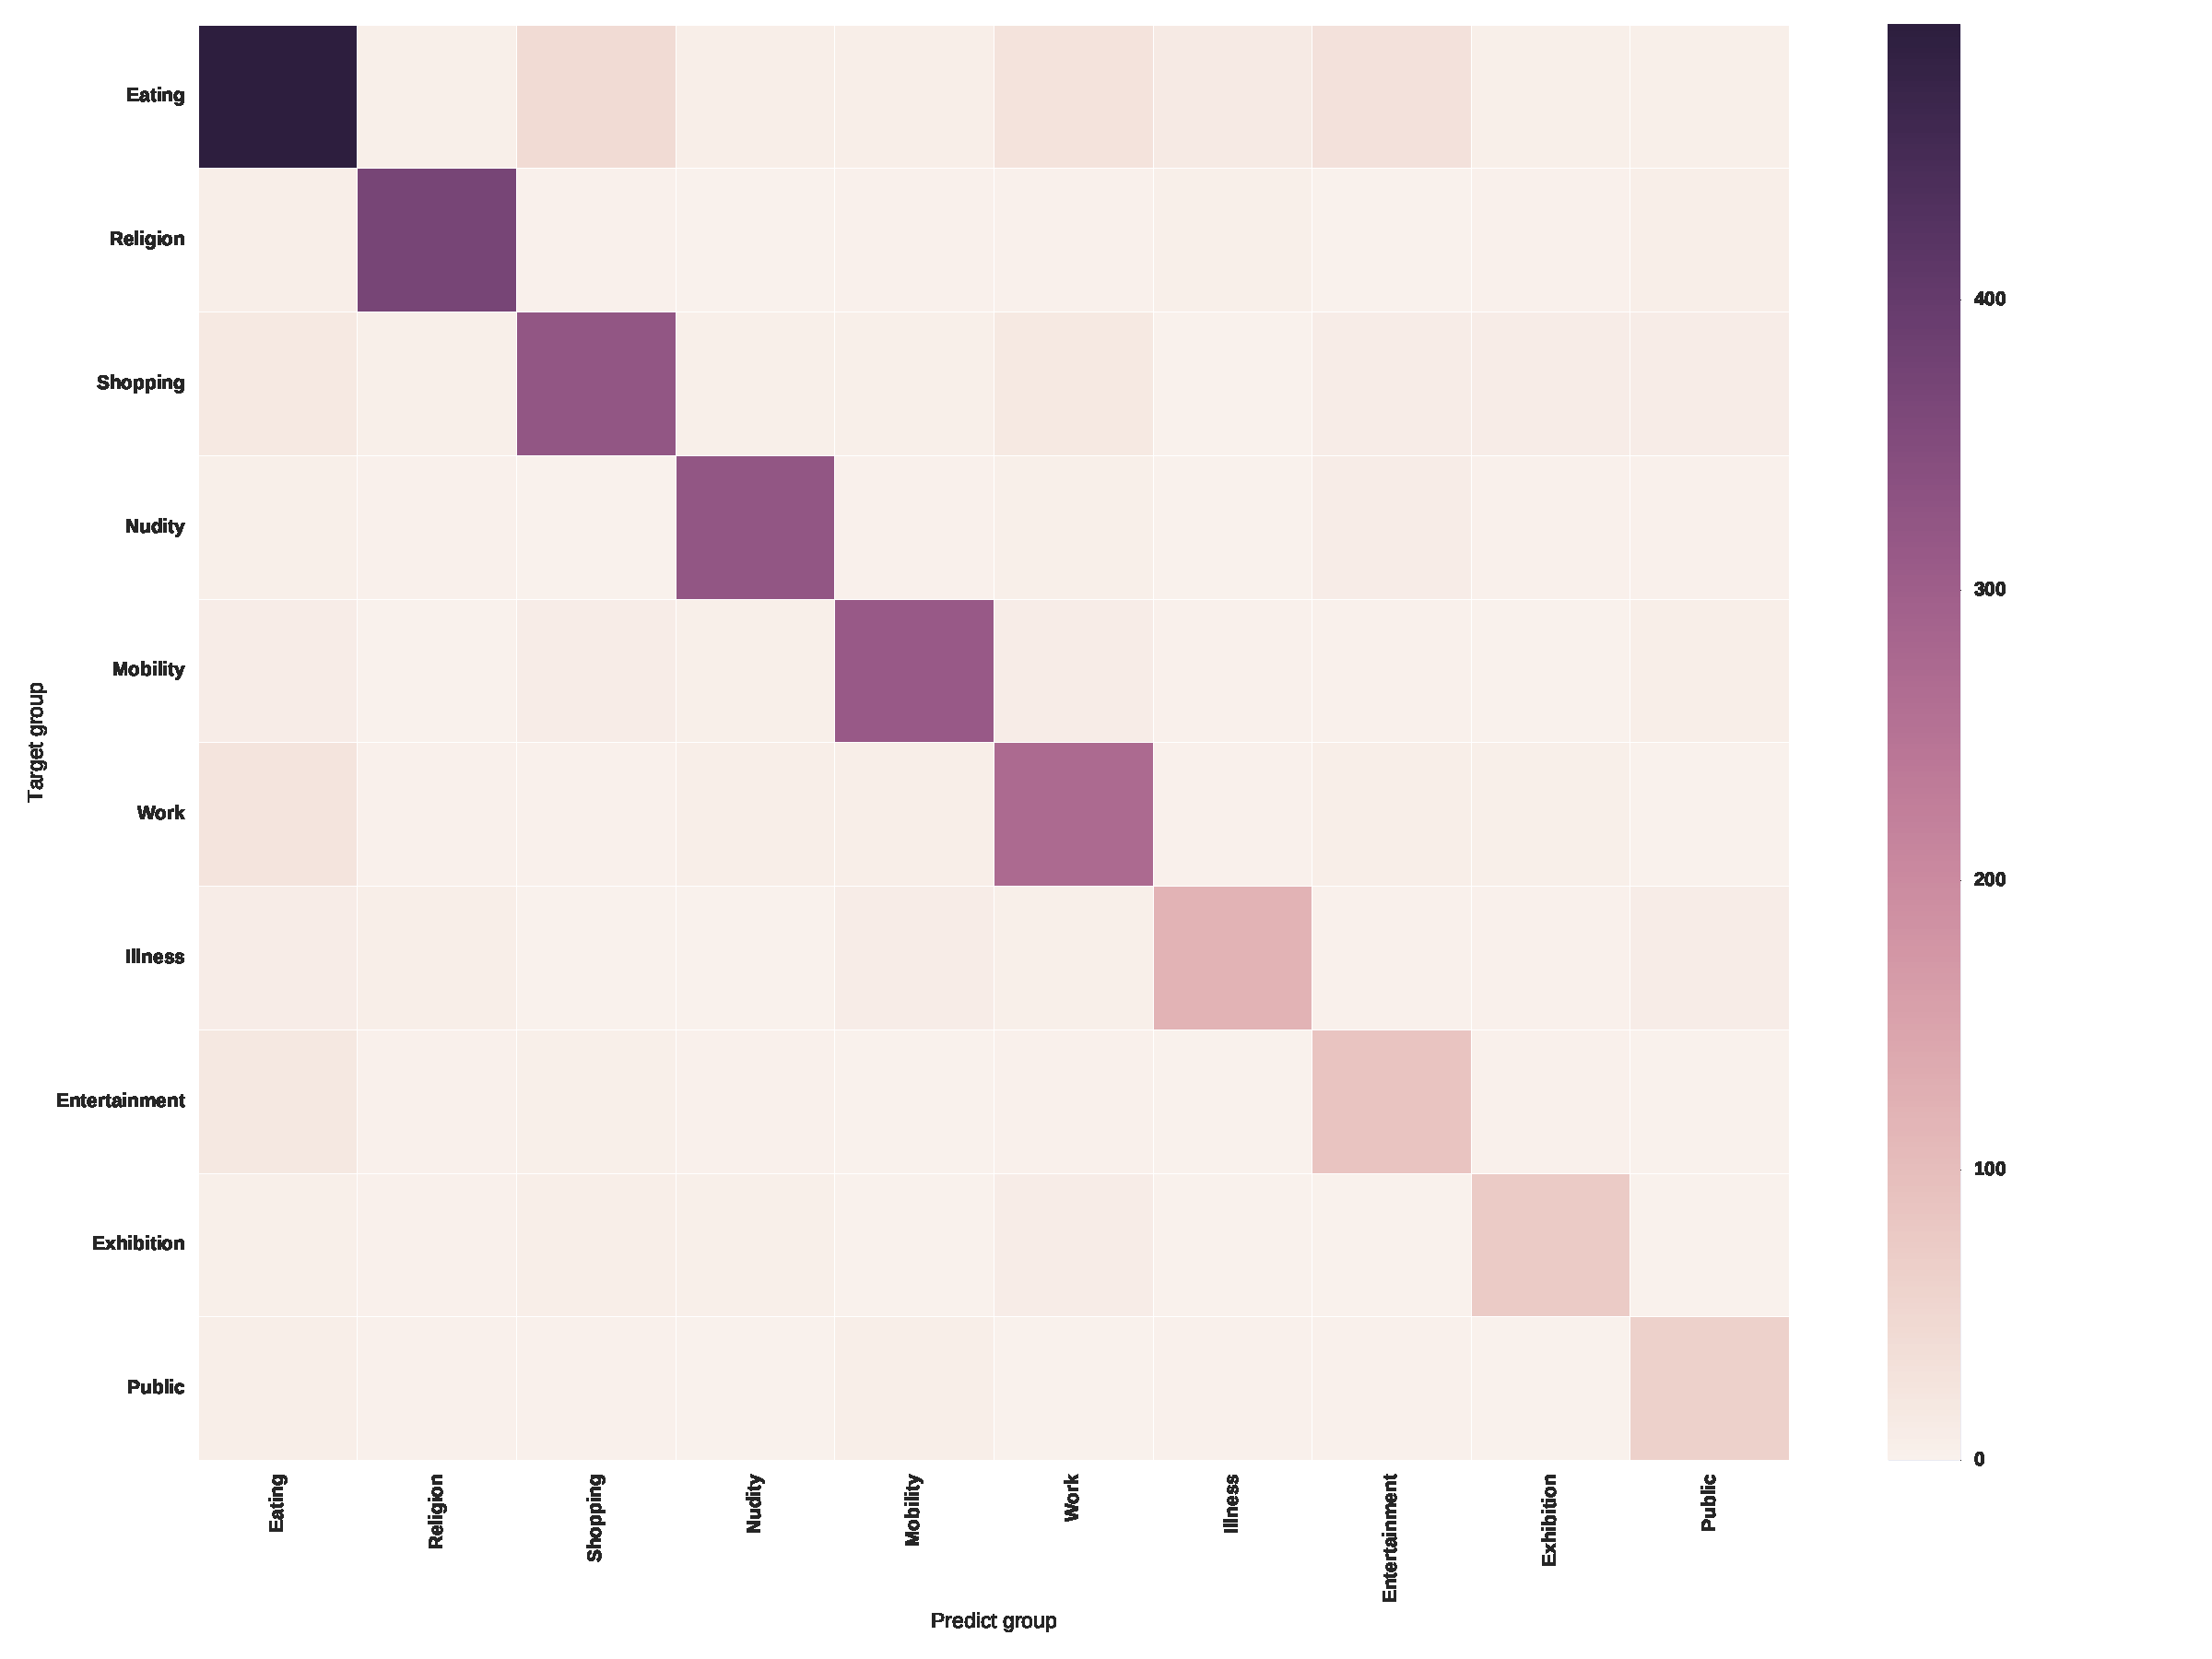
\includegraphics[width=0.6\textwidth]{figure/ch4-scnGrpConfu.pdf}}
    }
    \caption{Confusion matrices for category prediction (left) and group prediction (right).}
    \label{fig:ch4-scnconfumat}
\end{figure}



\subsection{Face Recognition}
Like scene classification, we select a pre-trained model for face recognition task. More specifically, the pre-trained model will serve as face feature extractor, and we will update the face classifier whenever new users register in Cardea and upload their face features. There are already many deep neural networks deployed in commercial products, like Megvii's Face++~\cite{zhou2013extensive}, Facebook's Deepface~\cite{taigman2014deepface}, Google's Facenet~\cite{schroff2015facenet}, Sensetime's Deepid~\cite{sun2015deepid3}. OpenFace~\cite{amos2016openface} is an open source project that is gaining attentions in recent months, it is based on Torch~\cite{links:torch7}. Because Cardea's other modules are under Caffe framework, we limit our options on open sourced Caffe models. The models in our consideration are VGG face recognition model~\cite{parkhi2015deep} and Lightened CNN face recognition model~\cite{wu2015lightened}.

\begin{figure}[!htbp]
    \makebox[\textwidth]{
        \centering
        \raisebox{-0.5\height}{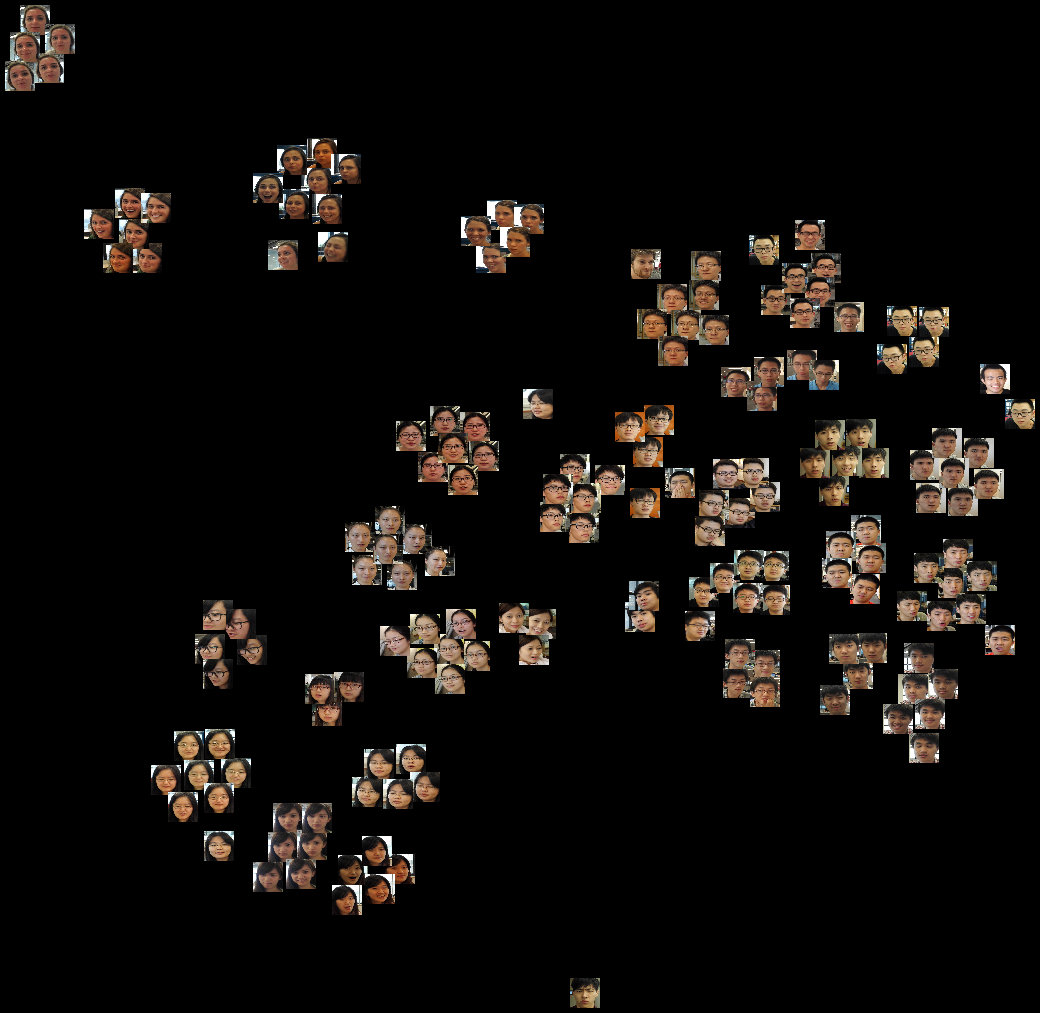
\includegraphics[width=0.6\textwidth]{figure/ch4-tsnevggfc8.png}}
        \raisebox{-0.5\height}{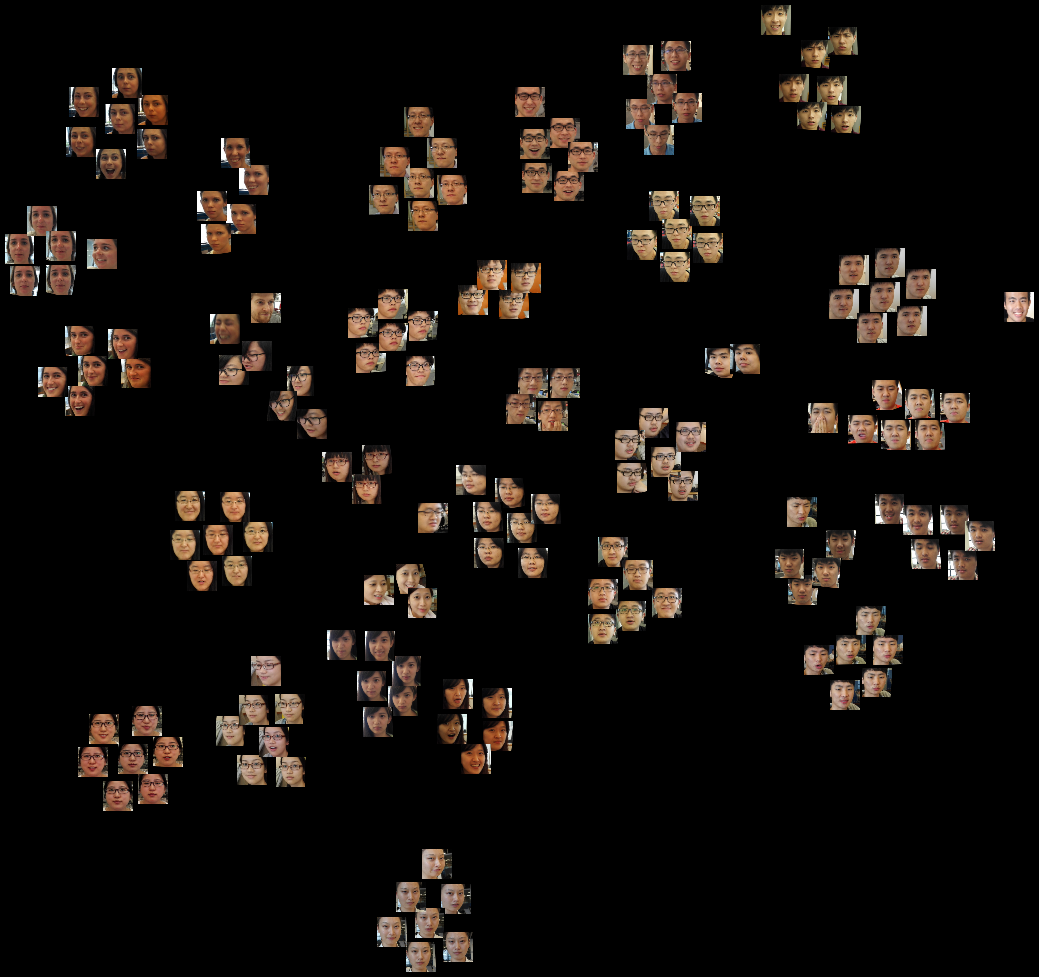
\includegraphics[width=0.62\textwidth]{figure/ch4-tsnemfmeltwise_fc1.png}}
    }
    \caption{t-SNE visualization of VGG \emph{fc8} layer features and Lightened CNN \emph{fc1} layer features.}
    \label{fig:ch4-tsnevggvsmfm}
\end{figure}

To compare performance of features extracted from the two models, we run t-SNE visualization~\cite{maaten2008visualizing} on the features of a small dataset we previously collected for emotion sensing. Fig~\ref{fig:ch4-tsnevggvsmfm} shows the t-SNE visualization result. It seems VGG feature and Lightened CNN feature have similar performance, at least on this small dataset. Though it is found that comparing to Lightened CNN model, VGG model is more robust to variations and its features show better transferability~\cite{ghazi2016comprehensive}, the model size is more than 500MB, 10 times bigger than Lightened CNN model. And the released VGG model has a feature dimension of 4096, while Lightened CNN model has a feature dimension of 256. Our experiment on different Android smartphones shows it takes 10 times longer to extract VGG features. Table~\ref{tbl-forwardingtime} shows the forwarding time we tested on different smartphones. It can be seen VGG model consumes much more memory that it can only run on phones with memory larger than 3GB. Due to above concerns, we use Lightened CNN model in our implementation.

\begin{table}[!htbp]
\centering
\caption{Time of single facial feature extraction and batch facial feature extraction (10 faces).}
\label{tbl-forwardingtime}
\begin{tabular}{lrrr}
\toprule
 & Xiaomi Mi 3W & Galaxy Note 4 & Xiaomi Mi 5\\
 & {\small Snapdragon 800} & {\small Snapdragon 805} & {\small Snapdragon 820}\\
 & {\small 2GB RAM} & {\small 3GB RAM} & {\small 4GB RAM}\\
 \midrule
1 VGG CNN & N/A & N/A & $\sim 2780$ ms \\
10 VGG CNN & N/A & N/A & $\sim 26740$ ms \\
1 Lightened CNN & $\sim 508$ ms & $\sim 330$ ms & $\sim 303$ ms \\
10 Lightened CNN & $\sim 6602$ ms & $\sim 3071$ ms & $\sim 2031$ ms \\
 \bottomrule

\end{tabular}
\end{table}


\subsubsection{Detection and Alignment}
Lightened CNN model takes aligned face as input, requiring that the distance between midpoint of eyes and midpoint of mouth is 48, and $y$ value of midpoint of eyes is 40, as shown in Fig~\ref{fig:ch4-facedetalign}. We use OpenCV's haar cascade~\cite{links:opencv,viola2001rapid} frontal face detector. The limitation it brings to Cardea is only frontal faces will be detected and recognized. We set \emph{minNeighbors} (the parameter specifying how many neighbors each candidate rectangle should have to retain it) to be 3 to ensure a relative high recall for face detection. To remove false positive, we further apply skin color filter (range $[0, 48, 60] - [30, 255, 255]$ in HSV color space) on retained rectangles. Following that, we use Dlib library's HOG~\cite{links:dlib,dalal2005histograms} based face detector as a second stage filter. Note that Dlib's face detector has higher accuracy comparing to OpenCV's face detector, but is much slower if applied directly on a high resolution image, therefore it is used as a filter on small rectangular areas. Dlib's facial landmarks detector~\cite{links:dlibfacepose} is also used in later face alignment stage, it can detect 68 facial landmarks~\cite{links:dlibfacelandmarkspos, links:dlibfacelandmarkscoords}. With the detected landmarks and required alignment condition about inputs to the CNN model, we can calculate the homography matrix that is finally used to align faces. The steps for detection and alignment is shown in Fig~\ref{fig:ch4-facedetalign}, and we implemented it as a JNI library for Android platform~\cite{links:facealignjni}.

\begin{figure}[!htbp]
    \centering
    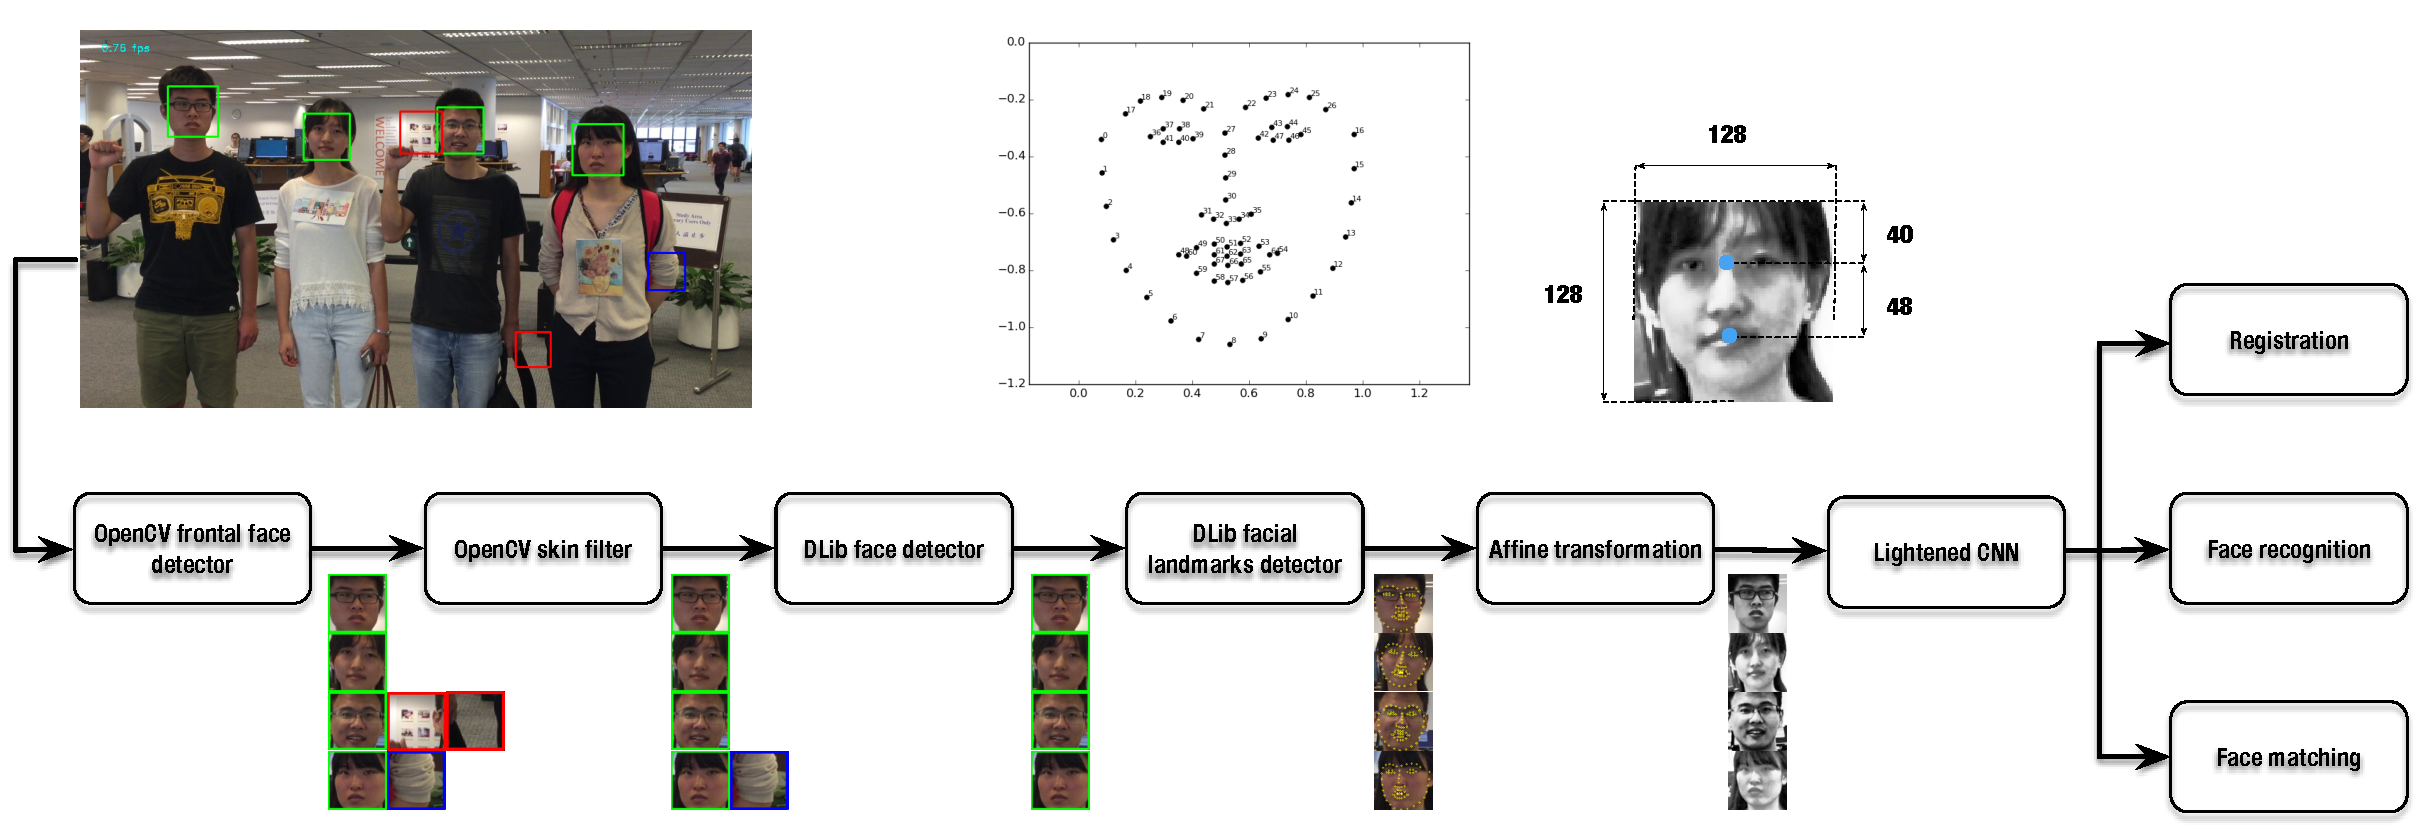
\includegraphics[width=1.0\textwidth]{figure/ch4-facedetalign.pdf}
    \caption{Face detection and alignment workflow.}
    \label{fig:ch4-facedetalign}
\end{figure}

\subsubsection{Recognition}
All the facial features uploaded by registered users are used to train a classifier in the cloud server, using LIBSVM library~\cite{chang2011libsvm}. During prediction, we enable probability estimations $p_i, i\in{1, \cdots, N}$, where $p_i$ is the probability of being user $i$. For each facial feature, if $\max_ip_i \leq T_p$, then we treat it as from an unknown person who hasn't registered in Cardea, otherwise it is from the user who has the highest probability and his privacy preference will be fetched for further processing. Threshold $T_p$ is an empirical parameter, a proper value of $T_p$ makes sure registered users are recognized correctly, and non-registered bystanders are recognized as unknown person. It is dependant on the face database scale, but the proper value can always be found through cross validation.

\subsubsection{Matching}
Face matching occurs when a recognized user $A$ has also specified and uploaded features of person $B$ with whom he doesn't want to be captured, it is to determine whether $B$ also appears in this captured image. Note that $B$ is not necessarily a registered user of Cardea. It is required that $n_B$, the number of $B$'s facial features uploaded by $A$ should be more than $10$. A simple way is pointing the camera on $B$'s photo but from different angles. Then for every detected face $C$ other than $A$ in the image, its feature $f_C$ will be compared with $n_B$ features of $B$ uploaded by $A$. $\mathtt{Cosine}$ similarity is used as distance metric. Among $n_B$ distances between $f_C$ and $B$'s features, we can calculate the ratio $r$ of distances which are shorter than a threshold $T_d$, if the ratio $r$ is higher than a threshold $T_r$, then $C$ and $B$ are the same person, thus $B$ appears with $A$ in the same image and $A$'s privacy will be protected. By tuning, we find $T_d \in (0.4, 0.6)$ and $T_r \in (0.4, 0.8) $ shows good enough performance. In Fig~\ref{fig:ch4-mfmsim}, we plot the distribution of distance between same person's Lightened CNN features and different person's Lightened CNN features. The features are extracted from all the faces in ORL face database~\cite{links:orlfacedb}, which consists of 400 images from 40 distinct subjects, 10 images per subject. Each subject has photos with different variations, such as: with/without glasses, open/closed eyes, and different facial expressions. It is obviously seen that distances between features of same person and features of different persons are well seprated, especially for the case of $\mathtt{cosine}$ similarity.

\begin{figure}[!htbp]
    \centering
    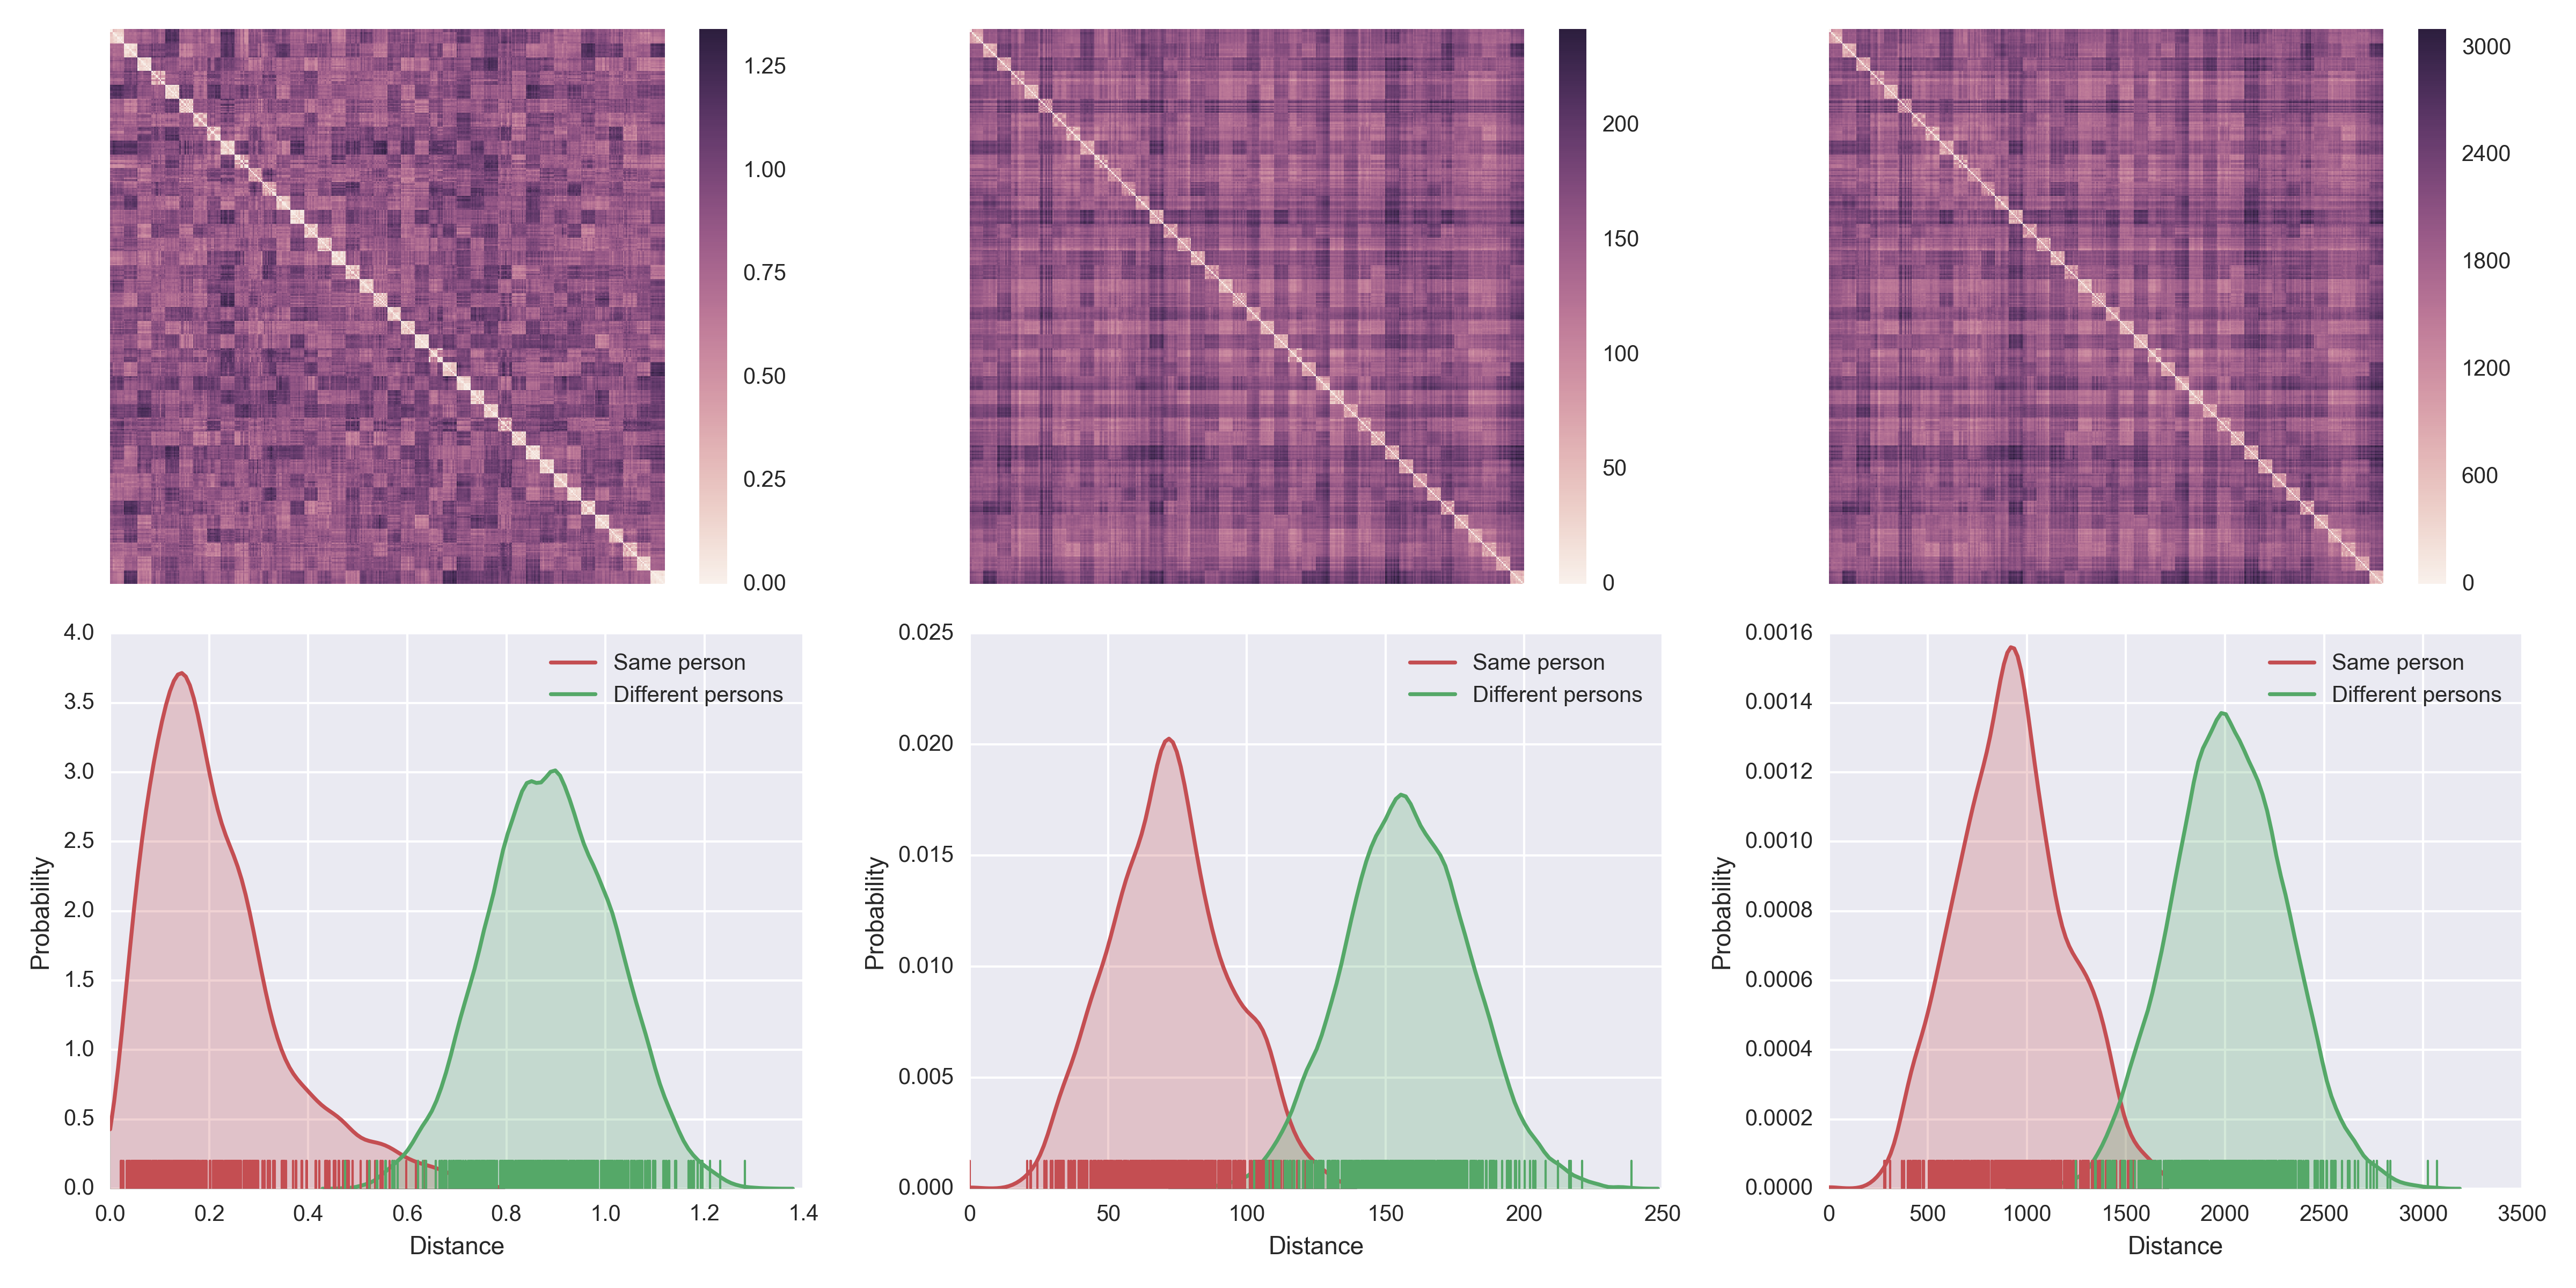
\includegraphics[width=1.0\textwidth]{figure/ch4-mfmsim.png}
    \caption{Distance matrix (top) and distance distribution (bottom) of Lightened CNN features using $\mathtt{cosine}$ similarity (left), $l_1$ norm (center) and $l_2$ norm (right).}
    \label{fig:ch4-mfmsim}
\end{figure}


\subsection{Gesture Recognition}
In Cardea, ``yes'' (\vcenteredinclude{figure/ch4-yesgesticon.png}) and ``no'' (\vcenteredinclude{figure/ch4-nogesticon.png}) gestures have the highest priorities and are used to temporarily overwrite privacy preferences. To recognize gestures in real world images, the first step is detection of hands, and it turns out to be the most challenging part in this sub task. Skin color based hand detector will fail dramatically in images with cluttered background. A much more robust method will be using multiple proposals~\cite{mittal2011hand} based on hand shape, context, and skin color. However, it takes an extremely long time to detect hands in one image. Finally, we choose to use state-of-the-art detection framework faster R-CNN~\cite{ren2015faster} to train a gesture detector in an end-to-end manner.

\subsubsection{Data Preparing and Preprocessing}


VGG group has shared a comprehensive dataset of hand images collected from various different public image data set sources in~\cite{mittal2011hand, links:vgghanddataset}. It contains 5628 images, which is composed of 4069 training images, 738 validation images, 821 testing images respectively, each image is with annotations of hand bounding boxes. However, this dataset can only let us train a hand detector. To achieve the goal of recognizing gestures, there are two solutions in our consideration:

\begin{itemize}
\item First train a hand detector using this dataset, then train another hand gesture classifier using other commonly used gesture datasets and pipe them together.
\item Take this dataset as a subset of images with ``natural'' gestures, then prepare extra images with ``yes'' and ``no'' gestures including annotations by ourselves, and train a ``natural/yes/no'' gesture detector end-to-end.
\end{itemize}

The first solution is not an end-to-end solution, and the specific ``yes'' and ``no'' gestures may not be included in those standard gesture datasets, then we will still need to prepare our specific gesture dataset like in second solution. Therefore, we choose the second solution, based on the observation and also assumption that annotated hands in VGG's hand dataset are in natural relaxing modes, thus will not be treated as ``yes'' or ``no'' gestures. The annotations of VGG dataset are tilted rectangles shown as yellow ones in Fig~\ref{fig:ch4-gesturedataset}, we re-annotate the dataset using bounding boxes of the original annotations shown as blue rectangles.

We crawled 527 images with ``yes'' hand gestures, and 363 images with``no'' hand gestures. Note that in a crawled image, it may contain different types of hand gestures as shown in Fig~\ref{fig:ch4-gesturedataset}, which is not a problem so long as gesture types are annotated correctly (\emph{remind} that all gestures in VGG dataset are treated as ``natural'' class). These images are crawled from Google and Flickr image search with keywords such as ``victory sign'', ``stop gesture'', ``palm gesture'' and so on, many of them are focused on the hands thus don't contain many background pixels. We rescale these images in different scales and then pad zeros on rescaled images. In Faster-RCNN python implementation~\cite{links:pyfasterrcnn}, an input image is rescaled to around $1000\times 1000$ before fed to region proposal network. If without padding data augmentation step, the bounding boxes of hand gestures will be huge in many crawled images that are focused on hands, which makes the learned model not able to detect small hand gestures and also not perform well on the regression of large hand gestures. Another reason for the padding step is to counter data imbalance of three classes. After augmentation, we have a dataset of 13843 images, including 5628 images from VGG dataset, 4712 augmented images mostly with ``yes'' gestures and 3503 augmented images mostly with ``no'' gestures. Fig~\ref{fig:ch4-gesturedataset} shows some sample images with annotations from this composed dataset. We wrote a tool~\cite{links:imgannota} to annotate the crawled images.

\begin{figure}[!htbp]
    \centering
    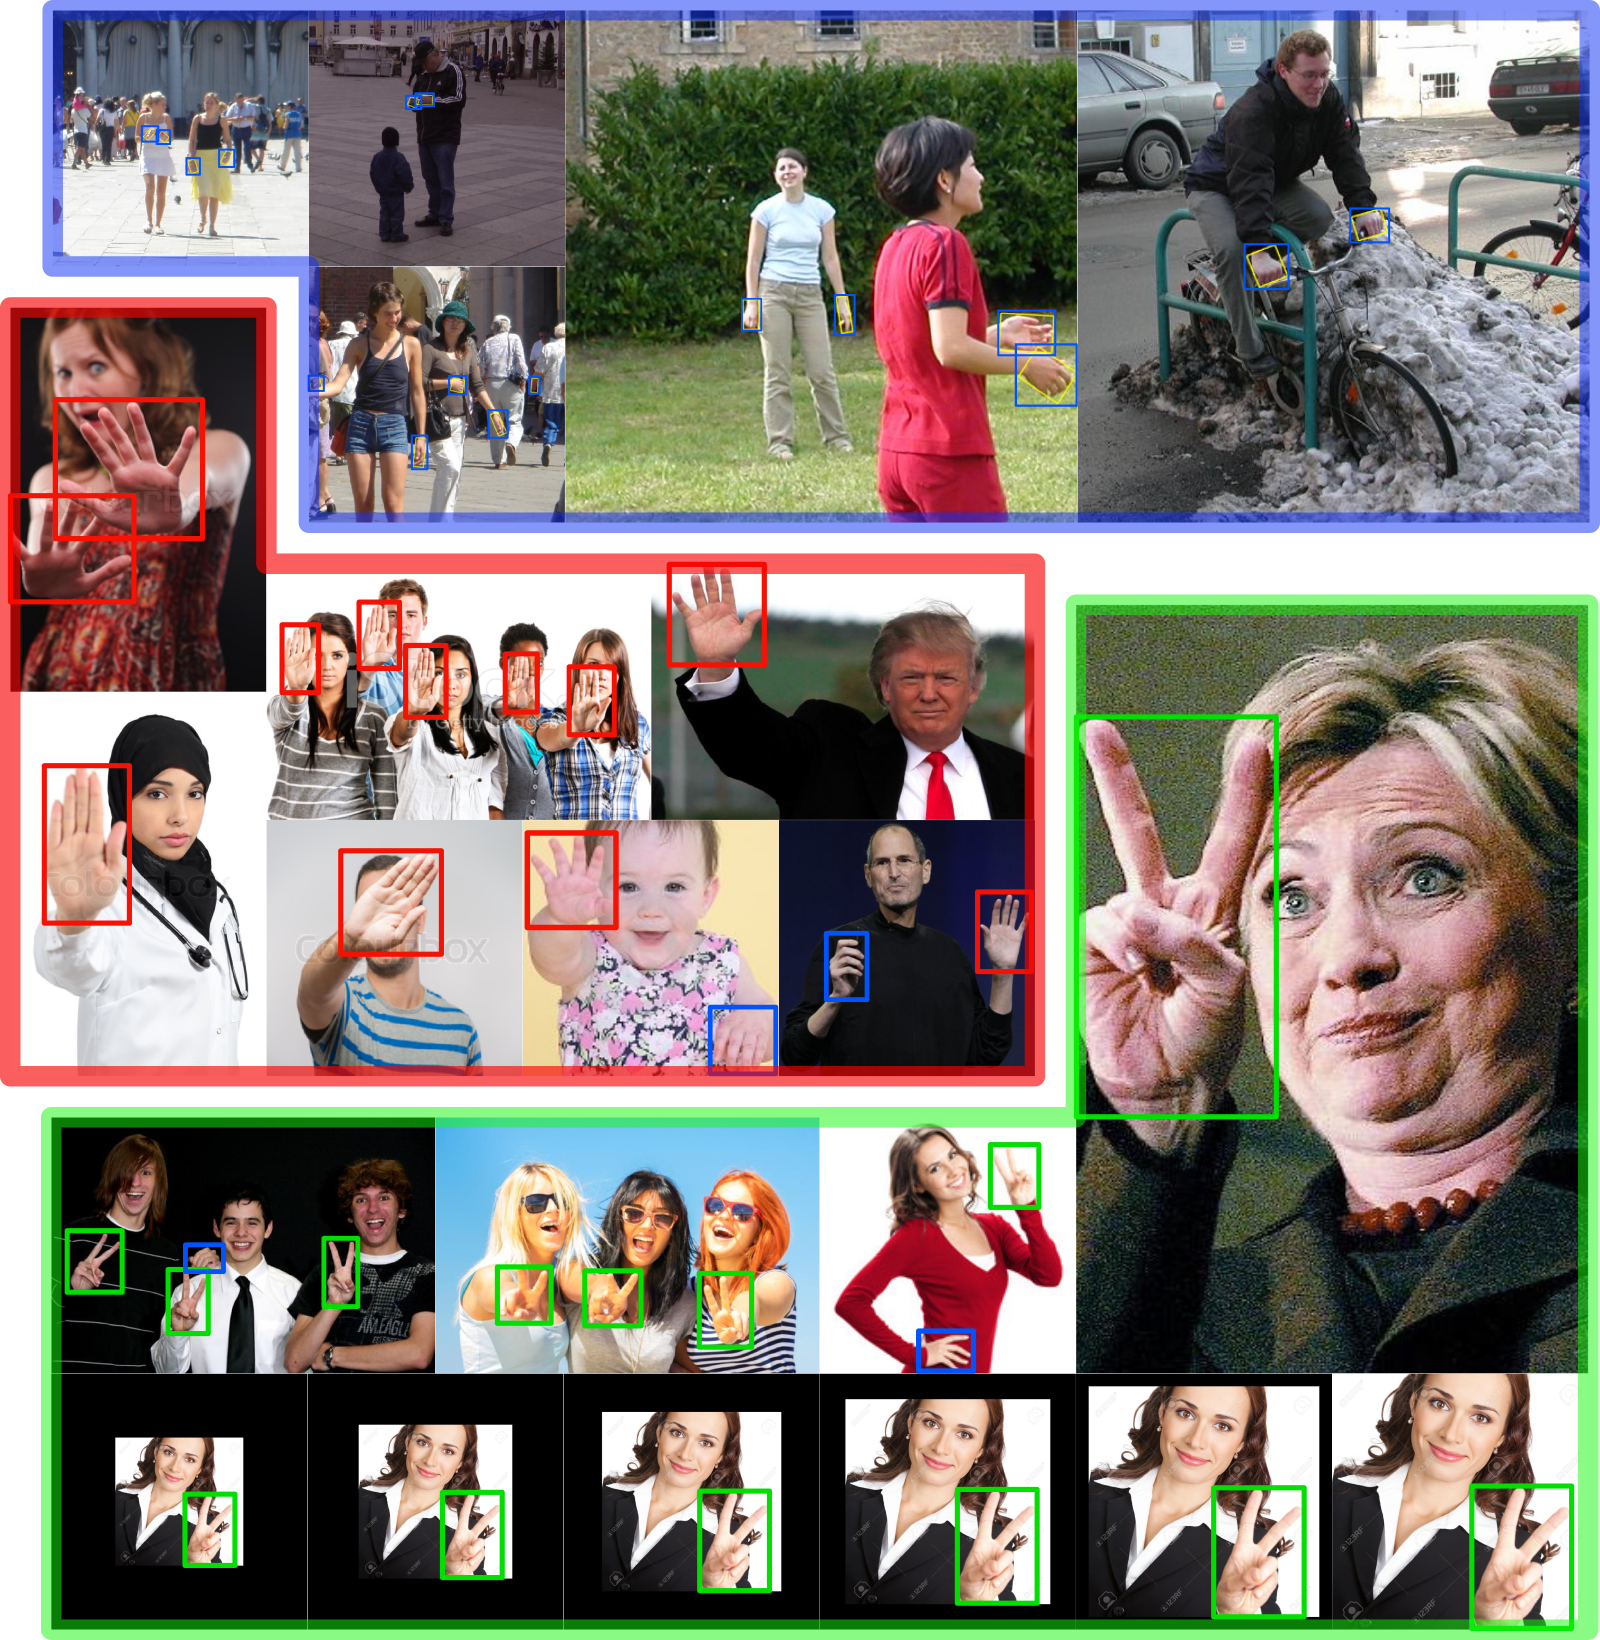
\includegraphics[width=0.8\textwidth]{figure/ch4-gesturedataset.png}
    \caption{Training hand gesture dataset composed of VGG hand dataset (top) and augmented crawled dataset (middle and bottom). Blue, red and green annotations denotes ``natural'', ``no'' and ``yes'' gestures.}
    \label{fig:ch4-gesturedataset}
\end{figure}

\subsubsection{Training Procedures}
Using the composed dataset, we fine-tune the \emph{conv3\_1} and up layers of VGG16 pre-trained model provided by Faster-RCNN library, jointly with region proposal layers and detection layers that are not part of VGG16 pre-trained model. Features from \emph{conv5\_3} layer of VGG16 network are shared between region proposal network (RPN) and Fast-RCNN~\cite{girshick2015fast} detection network, RPN uses them to generate proposals, and region of interest (ROI) pooling layer in detecting network uses them for bounding box regression and classification. There are two methods to train a shared feature extraction network. One is an alternating optimization method with following steps: \ding{182} Train an RPN $M_1$ initialized from VGG16 pre-trained model $M_0$, \ding{183} Generate training proposals $P_1$ using RPN $M_1$, \ding{184} Train Fast R-CNN model $M_2$ on proposals $P_1$ initialized from $M_0$, \ding{185} Train RPN $M_3$ from $M_2$ without changing convolutional layers, \ding{186} Generating proposals $P_2$ using RPN $M_3$, \ding{187} Train Fast R-CNN model $M_4$ on proposals $P_2$ initialized from $M_3$ without changing convolutional layers, \ding{188} Add $M_3$'s RPN layers to Fast R-CNN model $M_4$. Another method is an approximate joint optimization method by training with stochastic gradient descent as usual, which is easier, faster and achieves similar performance~\cite{links:pyfasterrcnn}, so we use the second training procedure.

\subsubsection{Prediction}
During prediction, we set Non-Maximum Suppression (NMS) threshold as 0.4 and confidence level threshold as 0.7. Figure~\ref{fig:ch4-gestpredictemp} shows some examples of gesture detection and recognition results in natural environment. It can be seen that the trained model can handle cluttered background such as in shopping environment, and indoor dark lighting condition. It is interesting to notice that bounding boxes for ``natural'' hands are bigger, reflecting the fact that we select re-annotated the VGG dataset for ``natural'' class using bounding boxes of the original annotations. The model has a good recall in terms of hand detection, however, its gesture recognition is sensitive to motion blur, palm angles and gesture size. We think the good recall of hands comes from the comprehensive VGG dataset, and the not so good recognition result is because the ``yes/no'' dataset we composed does not have a good quality because gestures are focused in many images, especially for ``no'' gestures, which is reflected by the observation that ``yes'' gesture recognition performs better than ``no'' gesture.

\begin{figure}[!htbp]
    \centering
    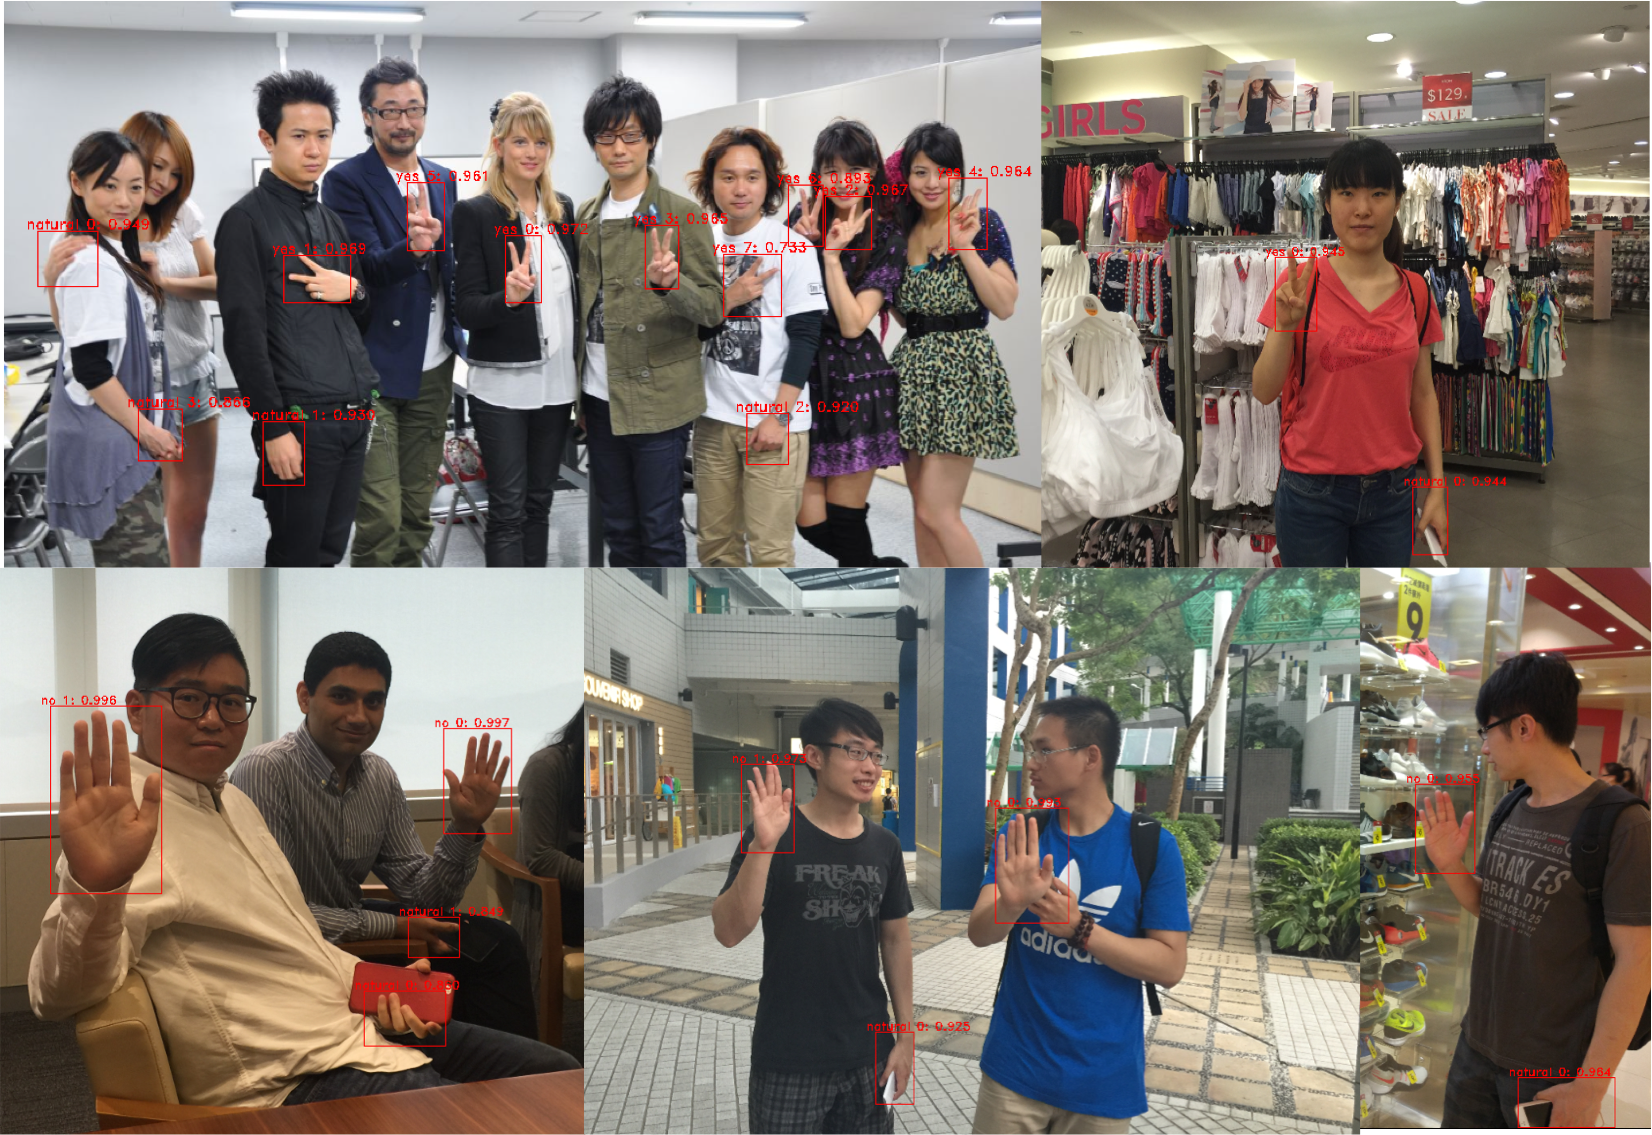
\includegraphics[width=0.8\textwidth]{figure/ch4-gestpredemp.png}
    \caption{Examples of gesture detection and recognition.}
    \label{fig:ch4-gestpredictemp}
\end{figure}



\section{System Integration}

\subsection{Deployment on Android}

Ideally, for a privacy control framework, we prefer a design that does not require cloud server and all the algorithms run locally on mobile devices. In the current design and implementation, cloud server exists mainly for two reasons: \ding{182} Storage center for profiles and hosting face recognition model; \ding{183} RPN in gesture recognition task is written in Python language, thus gesture recognition can not run on Android smartphones easily. However, these are not hard restrictions, possible improvements are discussed in Chapter 5.

The deployment of Caffe models for scene classification and facial feature extraction on smartphones is based on Caffe-android-library~\cite{links:caffeandroidlib}, we modified its code~\cite{links:caffeandroidlibzr} to support loading multiple Caffe models, batch feature extraction, and only forwarding to a specified layer during feature extraction, which saves useless computations from fully connected layers. There are other libraries for deploying neural networks on mobile, such as Torch-android~\cite{links:torchandroid} and MXNet~\cite{links:mxnetmobile}. The deployed scene classification model (based on AlexNet structure) has a size of 230MB, which is not small. However, its prediction is very fast, and can be easily fitted into the time slot when client is waiting response from cloud server. The facial feature extraction model (based on Lightened CNN structure) has a relatively bearable size of 33MB. Comparing to AlexNet, Lightened CNN model has smaller filter sizes, but with many more feature maps, therefore in run time, Lightened CNN model consumes about 1GB memory, which makes it not able to run on smartphones with less than 2GB memory as shown in Table~\ref{tbl-forwardingtime}. Possible ways to decrease model size and optimization of resource consumptions are also discussed in next chapter. Other lighter models we deployed on android include OpenCV face cascading model (less than 1MB) for face detection, and Dlib shape predictor (90MB) for facial landmarks detection.


\begin{figure}[b!]
    \centering
    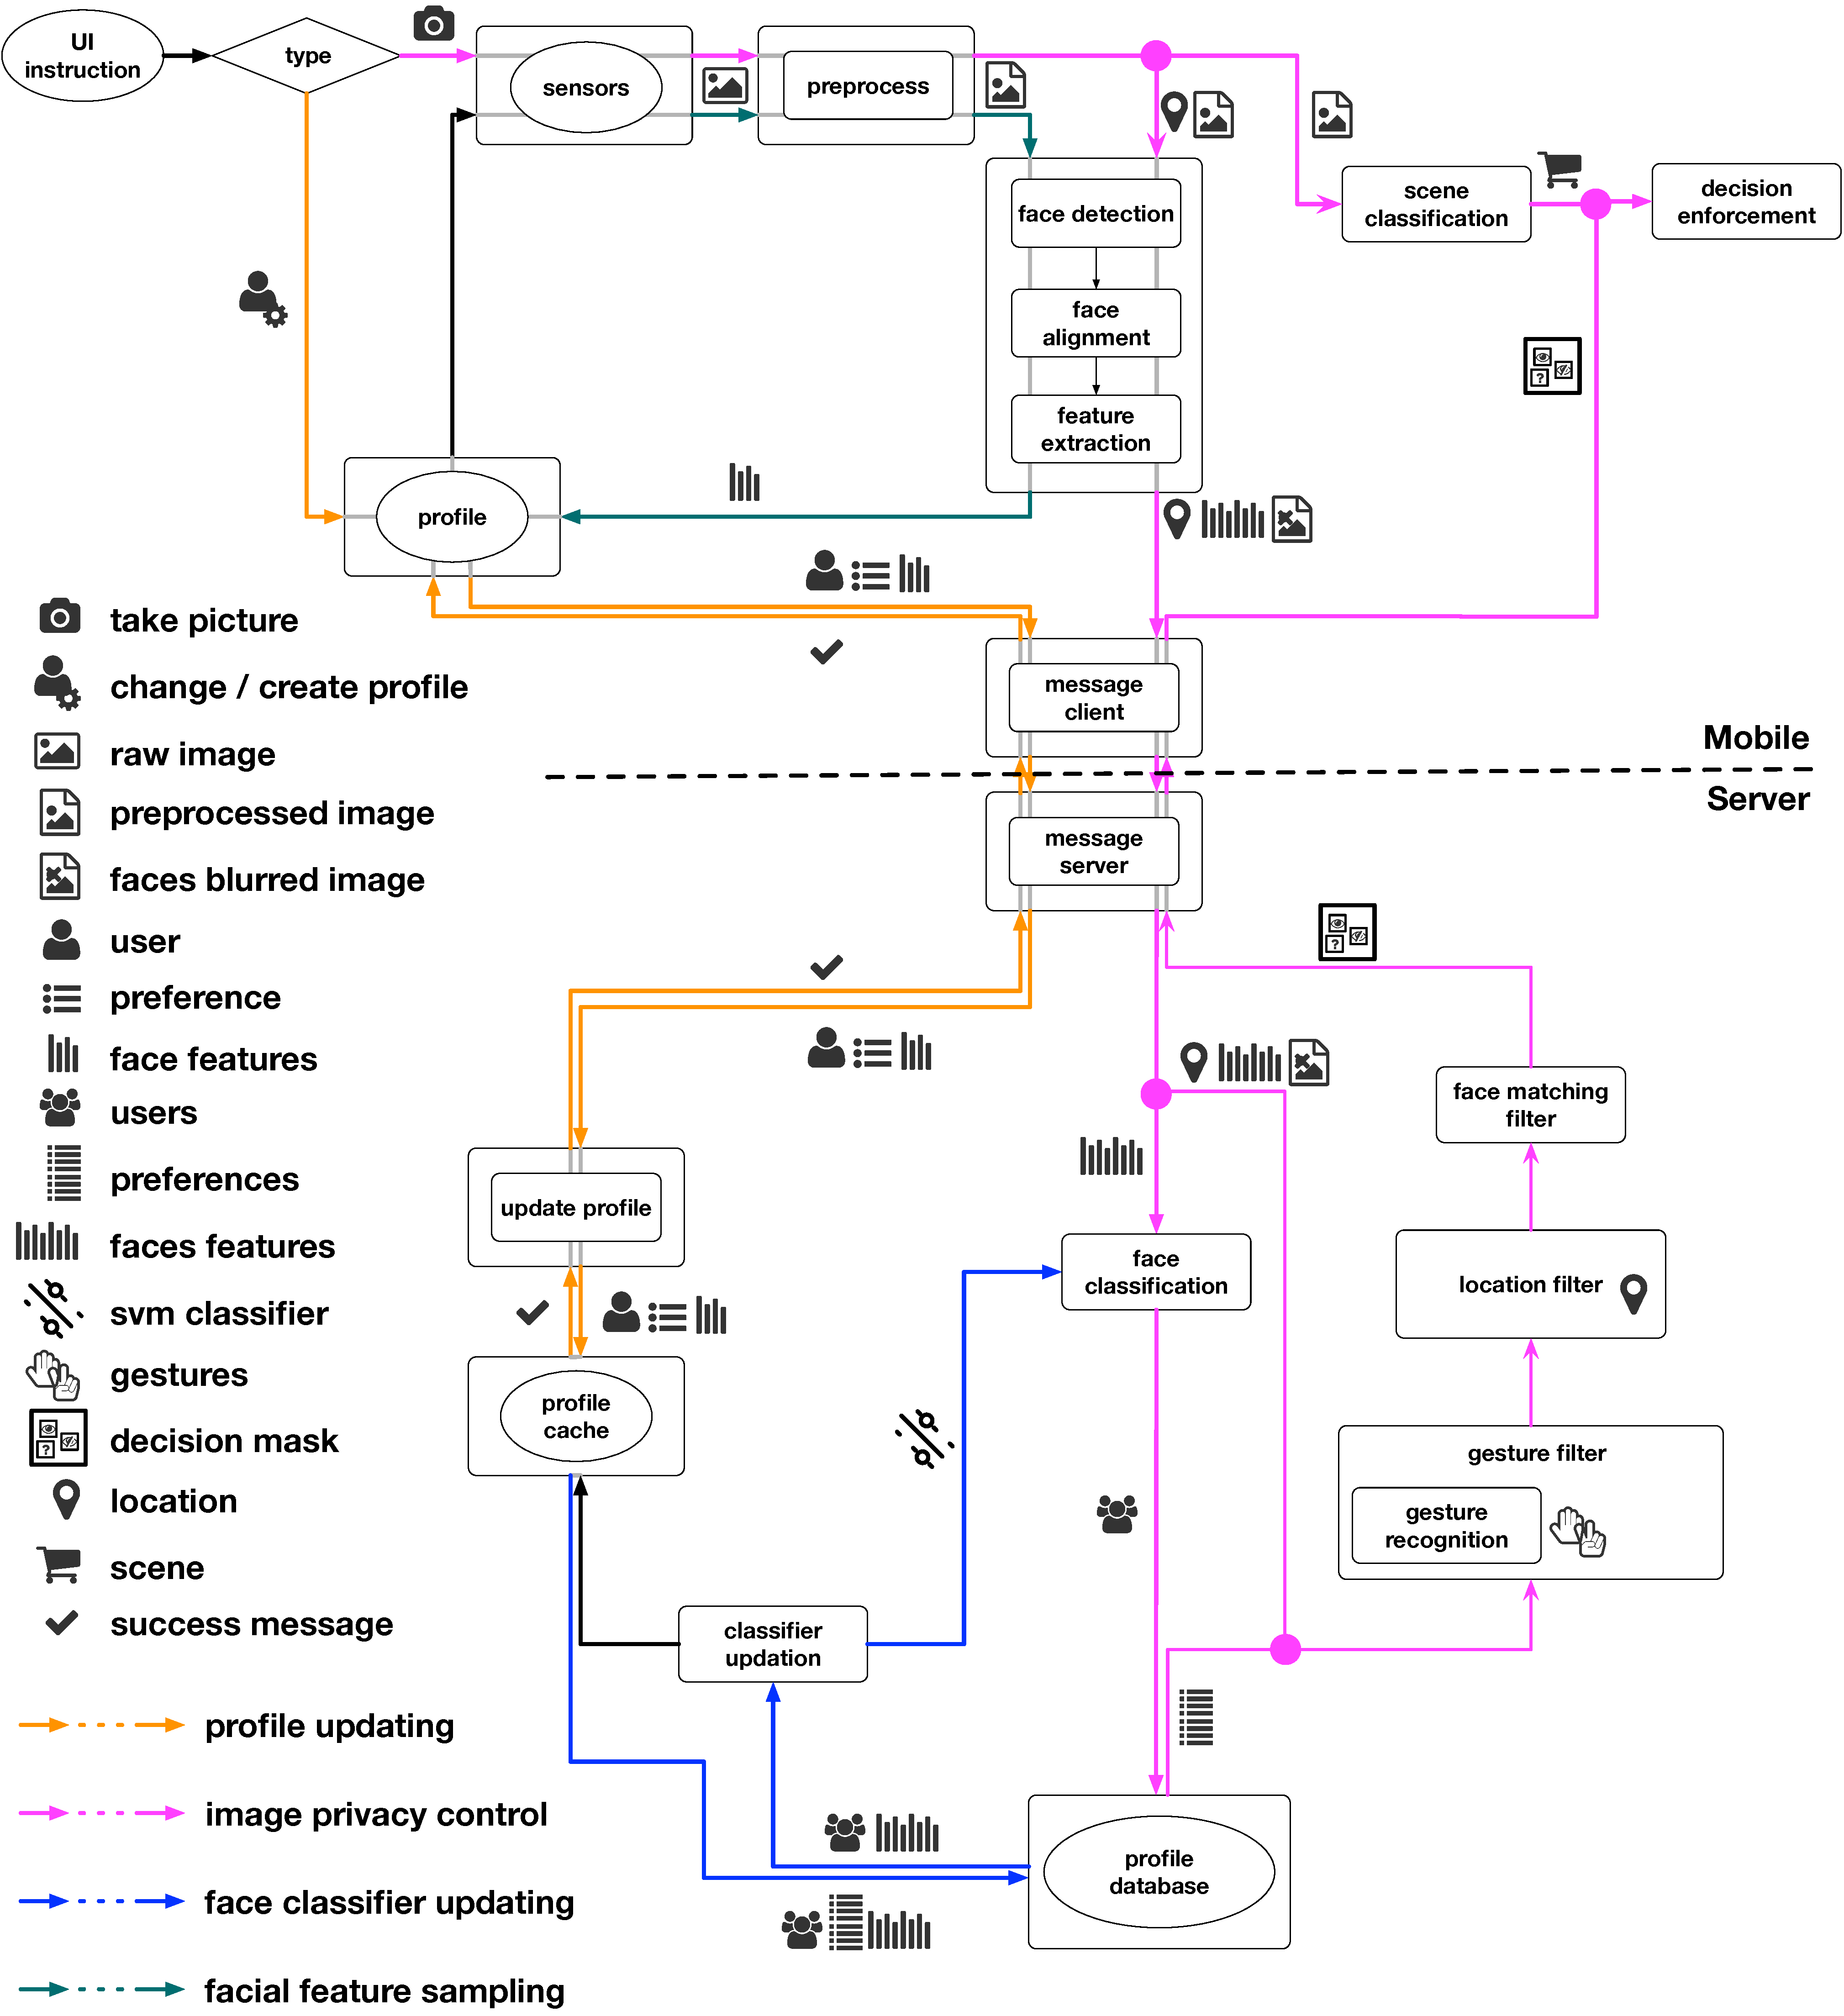
\includegraphics[width=0.6\textwidth]{figure/ch4-cardeadataflow.pdf}
    \caption{Dataflow of Cardea}
    \label{fig:ch4-cardeadataflow}
\end{figure}

\subsection{Dataflow and Integration}
Fig~\ref{fig:ch4-cardeadataflow} shows the detailed structure and dataflow of Cardea, which is mainly composed of the following steps (a demo video about the usage can be found in~\cite{links:cardeavid}):

\begin{description}[leftmargin=0cm]

\begin{figure}[!htbp]
  \makebox[\textwidth]{
    \centering
    \raisebox{-0.5\height}{
      \begin{subfigure}[b]{0.65\textwidth}
        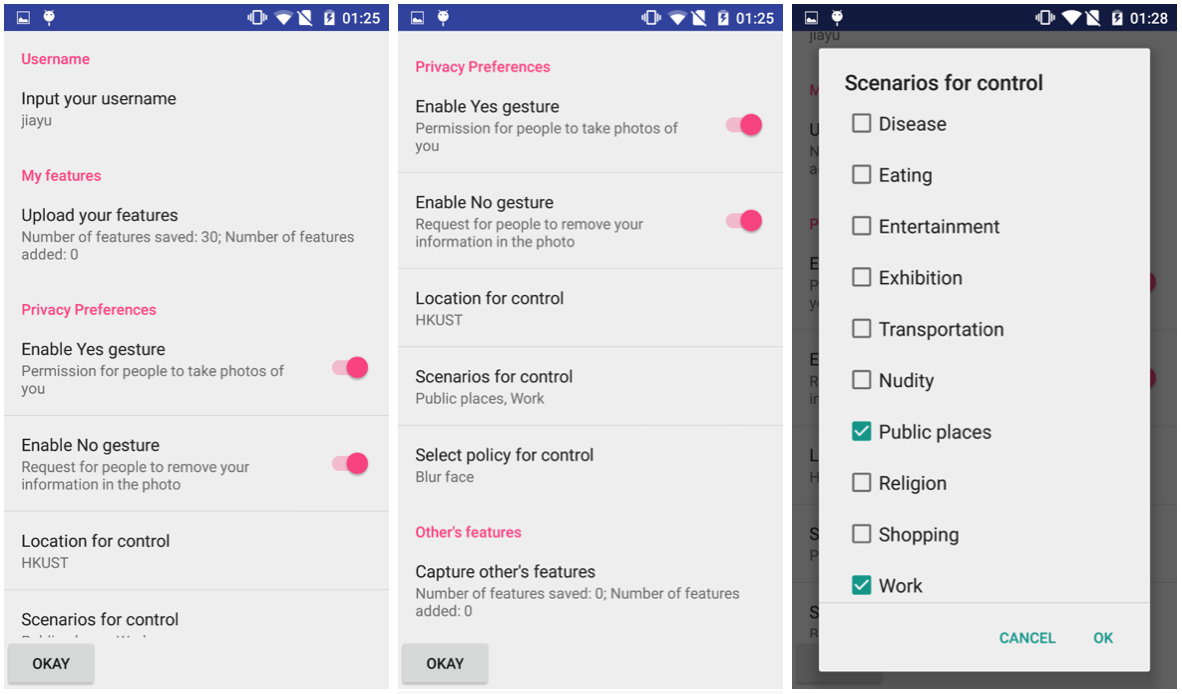
\includegraphics[width=\textwidth]{figure/ch4-reg.png}
        \caption{Registration and profile updating interface}
        \label{fig:ch4-reg}
      \end{subfigure}
    }
    \raisebox{-0.5\height}{
      \begin{subfigure}[b]{0.5\textwidth}
        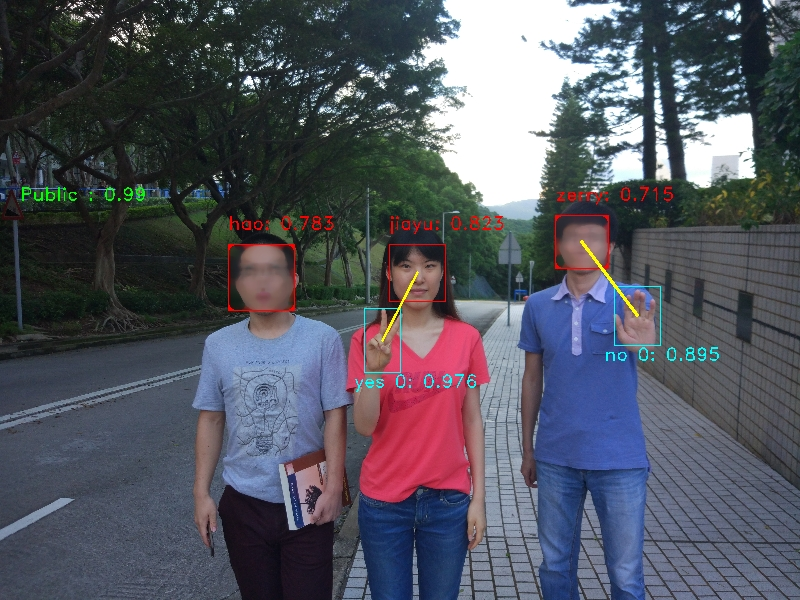
\includegraphics[width=\textwidth]{figure/ch4-allres.jpg}
        \caption{Privacy protection example}
        \label{fig:ch4-allres}
      \end{subfigure}
    }
  }
  \caption{Cardea user interface and privacy protection results. In (a), \textit{jiayu} registers as a Cardea user by extracting and uploading her face features. She specifies HKUST, two scene groups for privacy protection. She also enables ``yes'' and ``no'' gestures. In (b), a picture is taken in HKUST. 3 registered users, one ``yes'' and one ``no'' gesture are recognized. The scene is correctly predicted as ``Public''. \textit{jiayu}'s face is not blurred due to her ``yes'' gesture. Prediction probabilities are also shown in (b).}
  \label{fig:ch4-uires}
\end{figure}

  \item[{Registration and Profile updating:}] The interface provided to a bystander for registration and updating of his profile is shown in Fig~\ref{fig:ch4-reg}. He is able to select one or more scene categories, one location for control, as well as enable gestures or not. In two cases his facial features will be packaged with his privacy preferences: one is in registration time and the other is when he wants to update his facial features in the cloud. This registration and updating message will be send to server, if it is an updating message without feature updating, then his user profile in cloud will be updated immediately and he will receive a ``success'' notification, otherwise this message will be first buffered in a profile cache, and only after the next successful face classifier updating will he receive the ``success'' notification.

  \item[{Face classifier updating:}] In the server, the face classifier will be updated intermittently. For every time interval $\Delta T$, if there is cached messages that brings new facial features, it will \ding{182} block the queue of prediction messages from doing face recognition, \ding{183} merge profile cache with profile database, \ding{184} retrain a face classifer and \ding{185} unblock queued prediction messages.

  \item[{Image capturing:}] When a recorder uses Cardea to take a image, extracted facial features, GPS coordinate as well as face-blurred image will be packaged as prediction message and sent to server for processing. In the server side, after faces recognition and profiles retrieval, it will start the cloud part of decision making process for every face bounding box, after which what will be returned to the client side is a decision mask that specifies among all the detected faces, which should be blurred, which should be kept and which should be further determined based on the scene results calculated on the client side. In client side, while waiting for response from server it will calculate the scene result. With received decision mask, it makes final decisions on every face and enforces the privacy protection actions complied with everyone's preference.

\begin{figure}[!htbp]
    \centering
    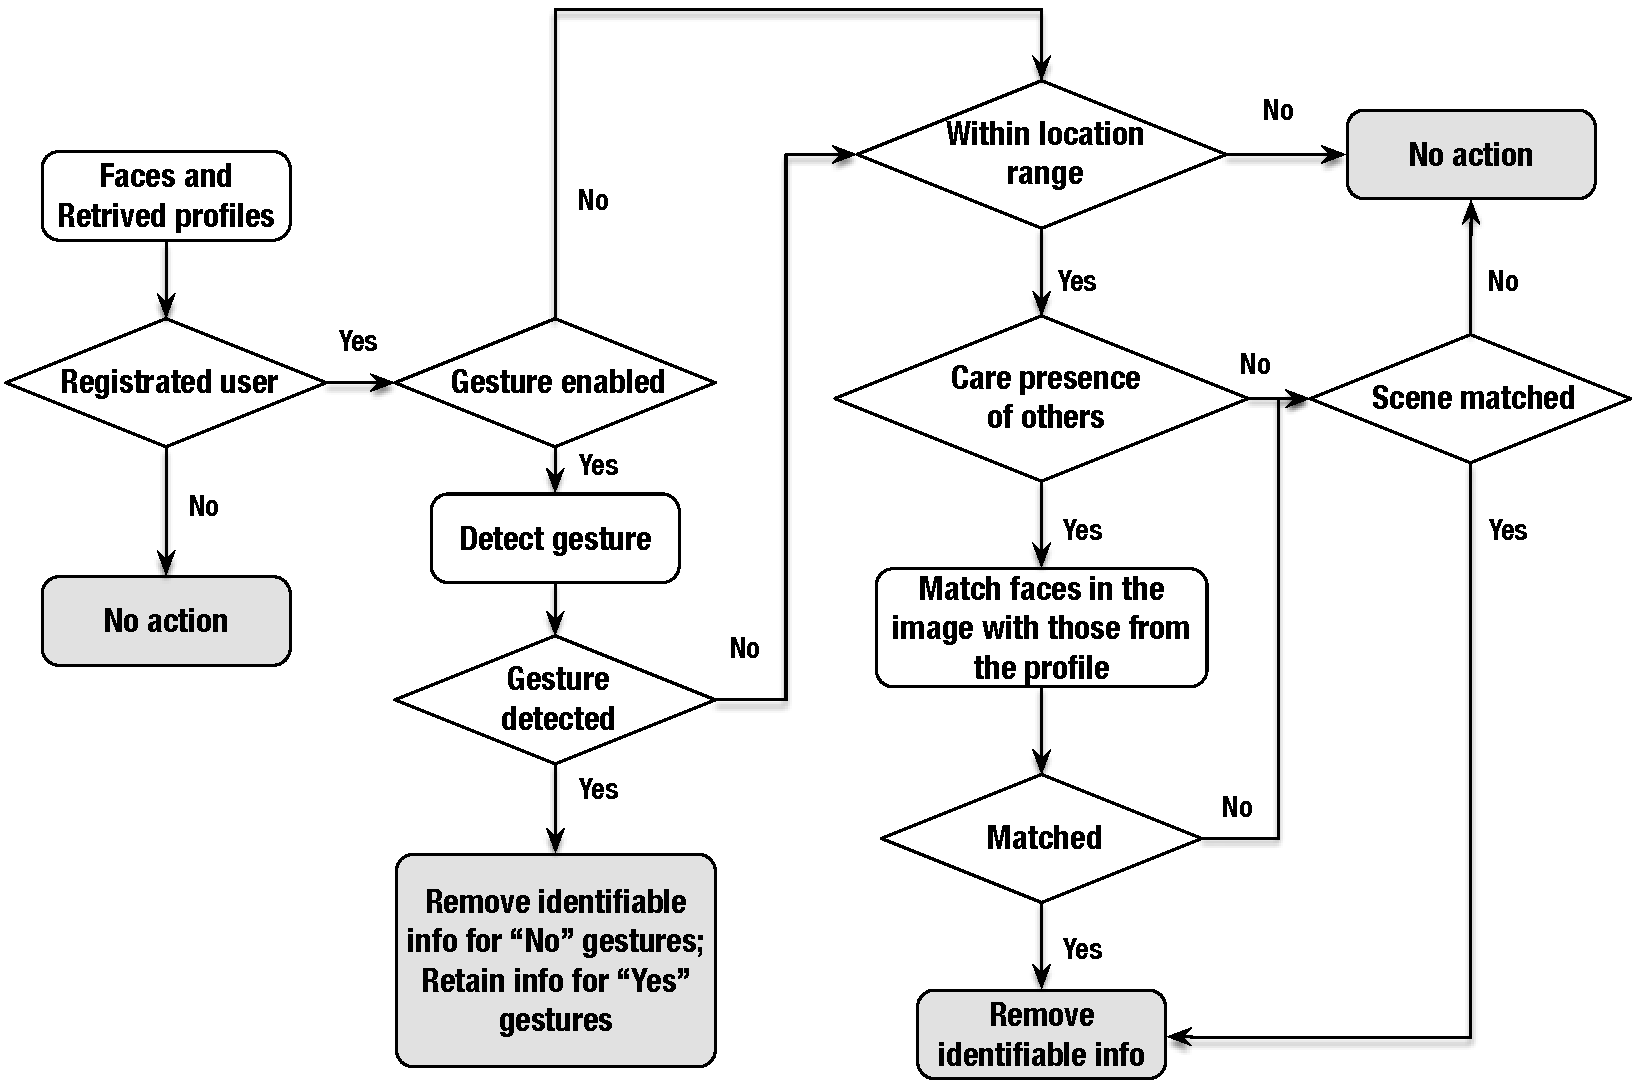
\includegraphics[width=0.6\textwidth]{figure/ch4-decisiontree.pdf}
    \caption{Steps of decisions about actions to be applied on detected faces.}
    \label{fig:ch4-decisiontree}
\end{figure}

  \item[{Decision making:}] Fig~\ref{fig:ch4-decisiontree} gives the detailed decision steps. Note that in this process, we need to match a detected gesture with the right face or people who issued the gesture, currently we simply take the nearest face of a detected gesture as the person who issued this gesture, thus it requires the user to put his hand near his face when sending ``yes/no'' gestures. As seen from the figure, when the detected face is recognized as a registered user, and context including location, scene, presence of other people and gesture matched with the user's profile, this detected face will be removed. An example is shown in Fig~\ref{fig:ch4-allres}. For other cases, the face will be kept but it may cause removal of other faces in the face matching step.


  \item[{Concurrent requests:}] To enable concurrent requests from different client apps, we implement multiple ``recognition'' workers to process the queued messages from all the clients, recognition results from different workers will be collected and put into a result queue, followed by multiple ``mailing'' workers to make decision masks and mail the decision masks back to corresponding blocked client threads. We tested with a server configuration - ``Intel i7-5820K CPU, 16GB RAM, GeForce 980Ti Graphic Card(6GB RAM)'' and the campus's Wi-Fi network, the time from start sending message to receive server's response is $1-2s$, depending on the message type. The total time from capturing moment to the enforcement of protection actions is $2-4s$, depending on how many faces detected. Most time is spent on facial feature extraction and message data transmission. Note that processing in the server side is relatively fast, gesture recognition of one image takes $200-300ms$, while the time spent on SVM face classifier and face matching is negligible. With 6GB GPU RAM, the server can serve 3 gesture recognition workers at the same time, supporting 5-10 concurrent requests. The implementation of Cardea is hosted in~\cite{links:cardeaproj}.

\end{description}


\section{Evaluation}

In this section, we present evaluation results along $3$ axes:

\begin{inparaenum}[\itshape 1\itshape)]
\noindent\item \textit{\textbf{vision micro--benchmarks}}, to evaluate the performance of different computer vision tasks, including scene classification, face recognition and matching, and hand gesture recognition. Note that when doing this evaluation, based on the categories shown in Table~\ref{tbl-scenecate}, we modify the scene categories and groups (add more categories and remove few categories and regroup them) hoping that it would cover more daily scenes (e.g. ``Exhibition'' group is removed). After this modification, we have $9$ groups composed of $98$ categories ($1.9$ million images) shown in Table~\ref{tbl-scenecateupdate}. We also retrain the scene classification model, and get 55\% category validation accuracy and 83\% group validation accuracy. {\textbf{All evaluations in this section are based on this new scene classification model.}} \\
\item \textit{\textbf{system overall performance}}, according to final privacy protection decisions and users' privacy preferences.\\
\item \textit{\textbf{runtime and energy consumption}}, which shows the processing time of each part, and energy consumed on one image.\\
\end{inparaenum}


\begin{table}[tb]
\centering
\caption{Nine general scene groups}
\label{tbl-scenecateupdate}
\begin{tabular}{llll}
\toprule
\textbf{Group name}  & \textbf{Abbreviatin}    & \textbf{Scenes \#}     & \textbf{Examples}   \\ \midrule
Shopping        &Sh & $20$            & clothing store, market, supermarket\\ \midrule
Travelling      &Tr & $9$             & airport, bus station, subway platform\\ \midrule
Park \& street  &Pa & $12$            & downtown, park, street, alley\\ \midrule
Eating \&       &Ea & $18$            & bar, bistro, cafeteria, coffee shop,\\
drinking        & &                 & fastfood restaurant, food court\\ \midrule
Working \&      &Wo & $9$             & classroom, conference center, library,\\
study           & &                 & office, reading room\\ \midrule
Scantily clad   &Sc & $12$            & beach, swimming pool, water park\\ \midrule
Medical care    &Me & $2$             & hospital room, nursing home\\ \midrule
Religion        &Re & $11$            & cathedral, chapel, church, temple\\ \midrule
Entertainment   &En & $5$             & amusement park, ballroom, discotheque\\ \midrule
\textit{All}    & & $\mathit{98}$   &   \\ \bottomrule
\end{tabular}
\end{table}

\subsection{Scene Classification}


We recruited $8$ volunteers and asked them to take pictures ``in the wild'' belonging to $9$ general scene groups. After manually annotating these pictures, we had $759$ images in total, with $638$ images in $9$ scene groups we are interested in. We then predict scene group for each image using the scene classification model we trained.

\begin{figure}[!htbp]
  \makebox[\textwidth]{
    \centering
    \raisebox{-0.5\height}{
      \begin{subfigure}[b]{0.5\textwidth}
        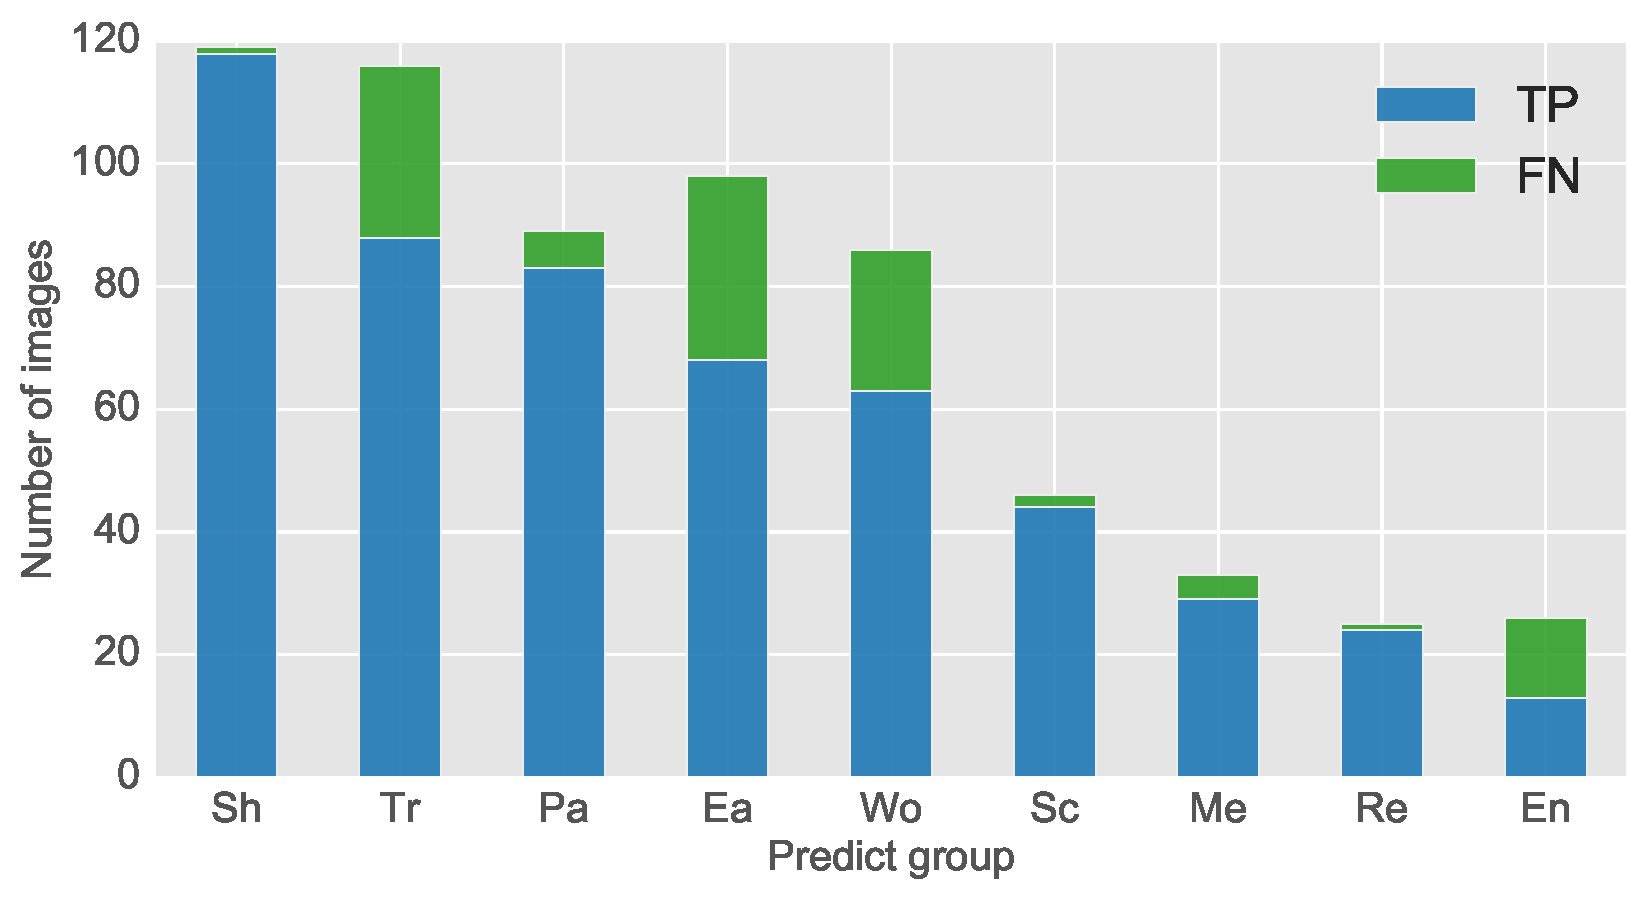
\includegraphics[width=\textwidth]{figure/ch4-scenerecall.pdf}
        \caption{Recall}
        \label{fig:ch4-scenerecall}
      \end{subfigure}
    }
    \raisebox{-0.5\height}{
      \begin{subfigure}[b]{0.5\textwidth}
        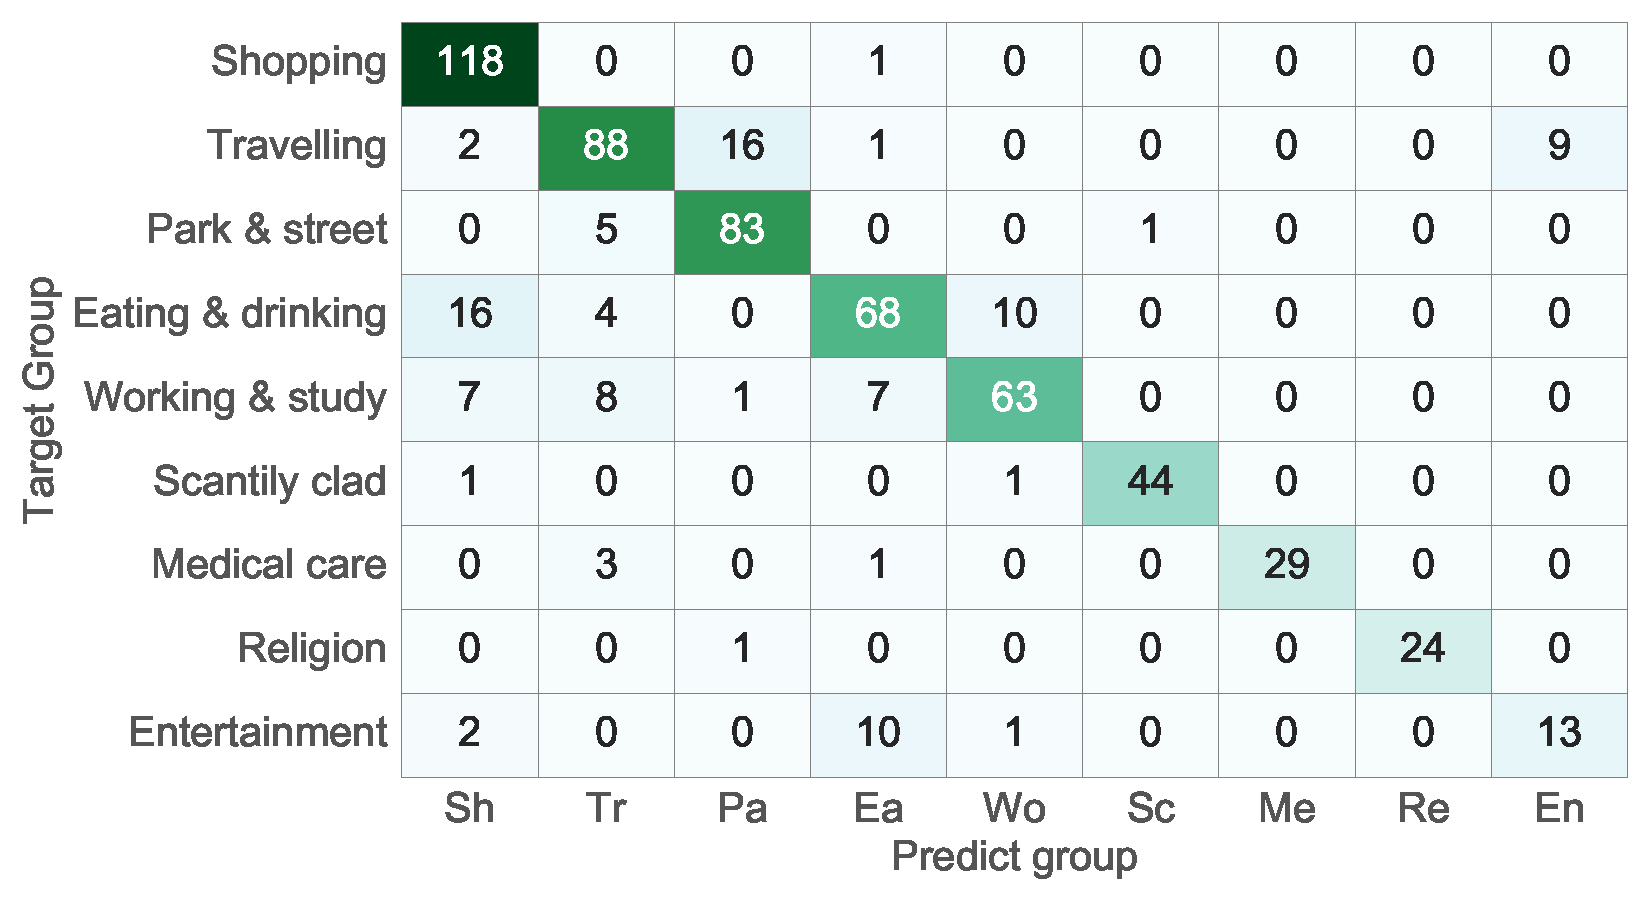
\includegraphics[width=\textwidth]{figure/ch4-sceneconfusion.pdf}
        \caption{Confusion matrix}
        \label{fig:ch4-sceneconfusion}
      \end{subfigure}
    }
  }

\caption{Scene classification evaluation results.}
\label{fig:ch4-sceneeval}
\end{figure}

The number of images and classification result of each group are shown in Figure~\ref{fig:ch4-scenerecall}. The true positives (TP) refers to images that are correctly classified, and false negatives (FN) are those classified as other scene groups. Overall, we can achieve {$0.83$} recall (TP/(TP+FN)), and $5$ scene groups are with recall more than $0.90$. It is worth mention that the recall of scene groups \textit{Scantily clad (Sc)}, \textit{Medical care (Me)}, and \textit{Religion (Re)} exceed $0.95$, which provides strong support to protect users' privacy in sensitive scenes.

We also give the detailed classification confusion matrix in Figure~\ref{fig:ch4-sceneconfusion}. It shows that most FN of \textit{Eating \& drinking (Ea)} are classified as \textit{Shopping (Sh)} or \textit{Working \& study (Wo)}, and most FN of \textit{Wo} are classified as \textit{Ea} or \textit{Sh}. The reason is that boundaries between \textit{Sh}, \textit{Ea}, or \textit{Wo} are not clear. For example, shopping malls have food courts, or people study in coffee shop. The same reason accounts for the confusion between \textit{Park \& street (Pa)} and \textit{Travelling (Tr)}. Moreover, for scene categories such as pub and bar, people may group them into \textit{Ea} or \textit{En}. Therefore, a safe way is to select more scene groups, for instance, both \textit{Ea} and \textit{En} when you go to a pub at night.

In general, the evaluation results from images captured ``in the wild'' demonstrate that most of scenes can be correctly classified, the performance is especially satisfactory for those sensitive scenes.


\subsection{Face Recognition and Matching}
We first select $50$ subjects from LFW dataset \cite{links:lfw} who has more than $10$ images as registered users. Note that subjects in the CASIA WebFace Database used to train the lightened CNN model do not overlap with those in LFW. For each subject, we extract at least $100$ face features form Youtube video to simulate the process of user registration. In total, we get $5042$ feature vectors. These features are then divided into the training set and validation set. In addition, we collect user test set and non--user test set to evaluate the face recognition accuracy. The user test set is composed of $511$ face feature vectors from online images of all $50$ registered users. The non--user test set consists of $166$ face feature vectors from $100$ subjects in LFW database whose names start with ``\textit{A}'' as non--registered bystanders.

\begin{figure}[!htbp]
  \makebox[\textwidth]{
    \centering
    \raisebox{-0.5\height}{
      \begin{subfigure}[b]{0.5\textwidth}
        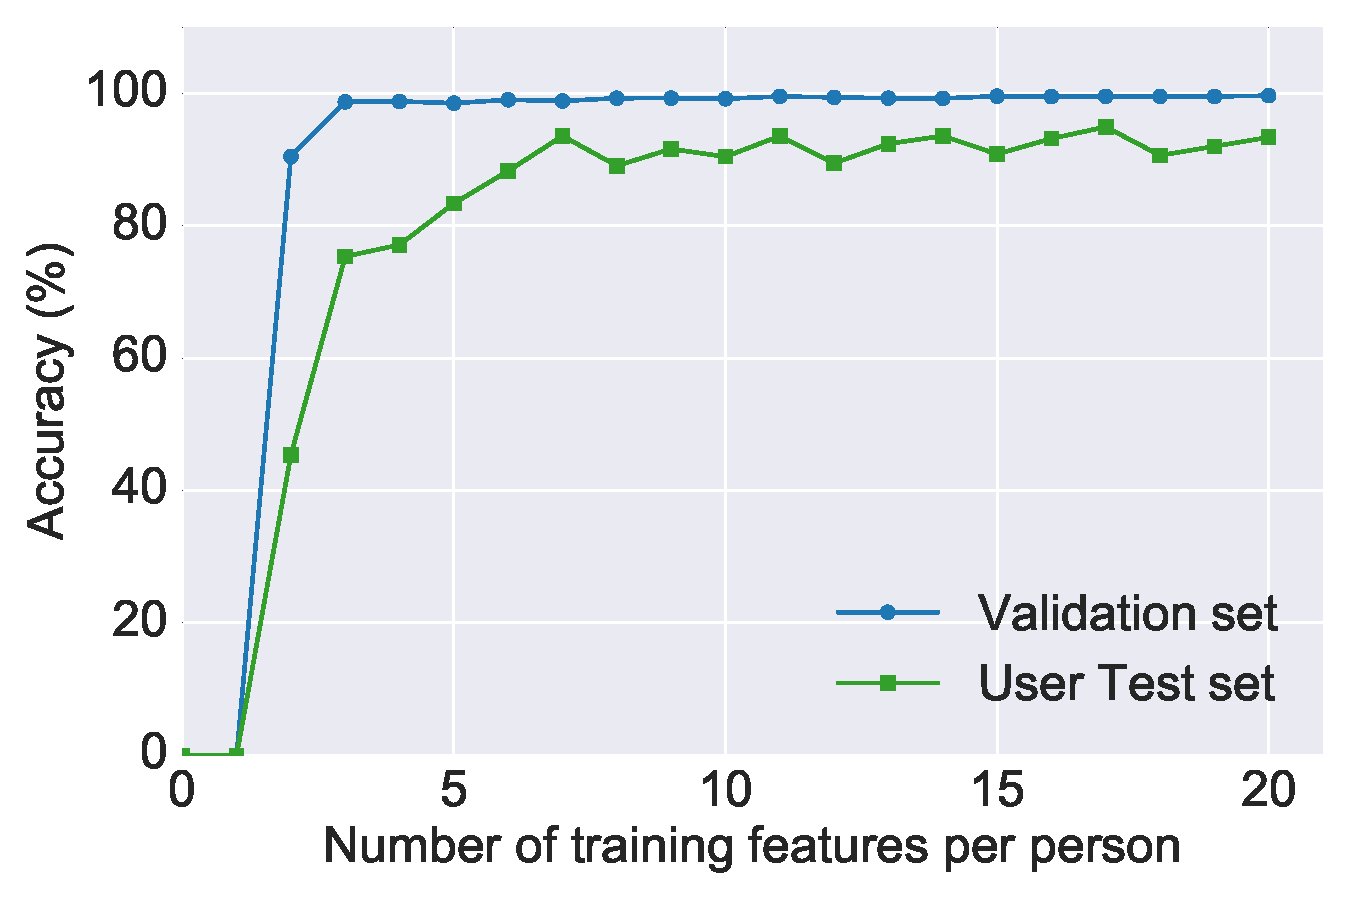
\includegraphics[width=\textwidth]{figure/ch4-accuracy-num.pdf}
        \caption{Training accuracy}
        \label{fig:ch4-accnum}
      \end{subfigure}
    }
    \raisebox{-0.5\height}{
      \begin{subfigure}[b]{0.5\textwidth}
        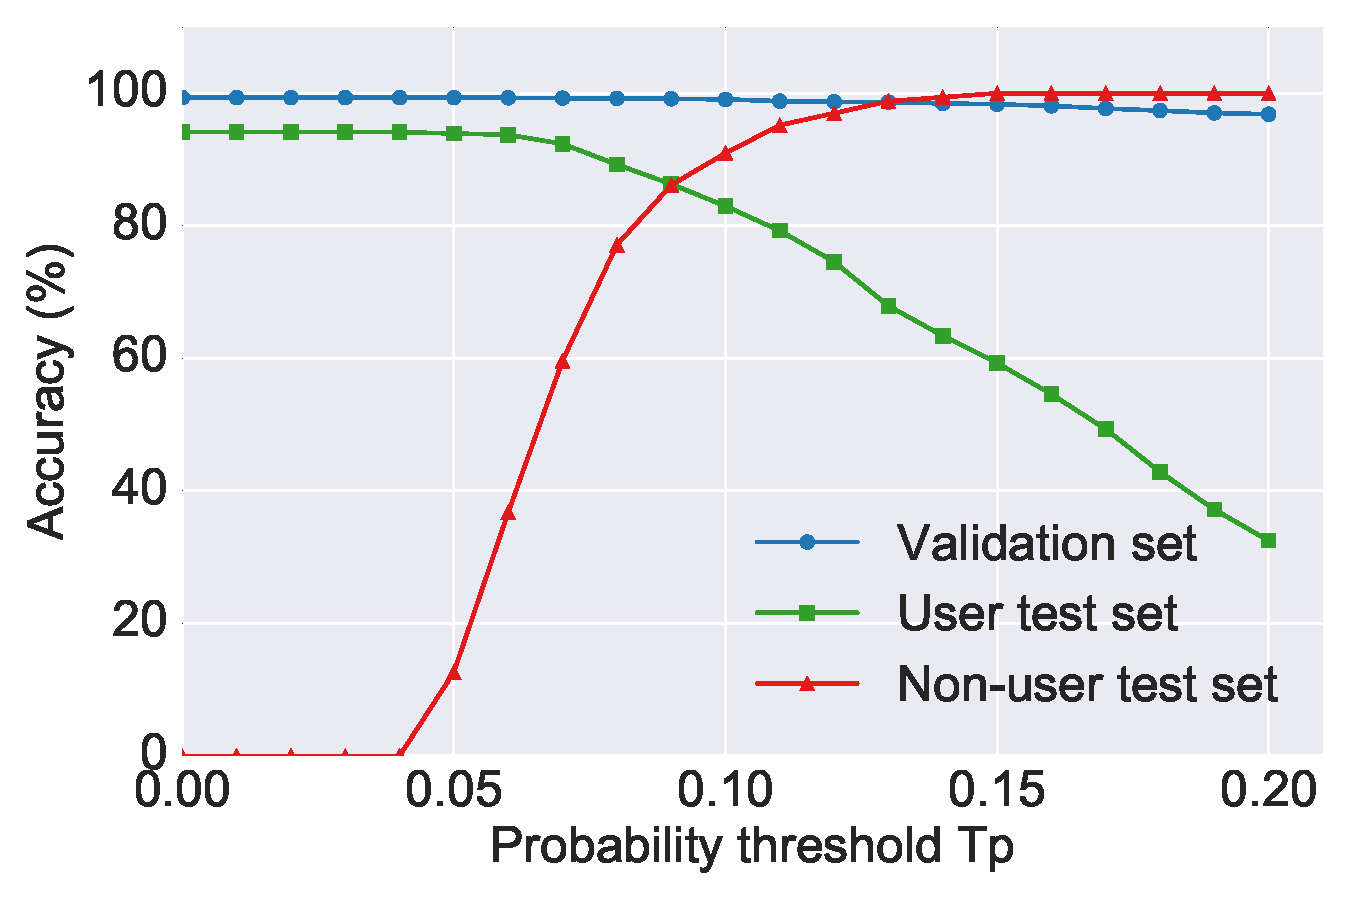
\includegraphics[width=\textwidth]{figure/ch4-accuracy-threshold.pdf}
        \caption{Testing accuracy with threshold $T_p$}
        \label{fig:ch4-accthreshold}
      \end{subfigure}
    }
  }
\caption{Face recognition accuracy.}
\label{fig:ch4-facereceval}
\end{figure}

Figure~\ref{fig:ch4-accnum} shows the recognition accuracy as to validation set and user test set with different numbers of features per person used for training. The accuracy refers to the fraction of faces that are correctly recognized. The results show the model trained with $10 \sim 20$ features per person can achieve near $100\%$ accuracy on the validation set and over $90\%$ accuracy on the user test set. Little improvement can be achieved with more training data. Figure~\ref{fig:ch4-accthreshold} shows the overall accuracy with probability threshold $T_p$. For non--user test set, the accuracy means the fraction of faces that are not recognized as registered users. As a result, the accuracy will increase for the non--user test set but decrease for the validation set and user test set when $T_p$ goes up. To make sure that registered users can be correctly recognized, and non-registered users will not be mistakenly recognized, we choose $T_p$ to be $0.08 \sim 0.09$, which achieves over $80\%$ recognition accuracy for both users and non--users. It is worth mentioning that the proper value of $T_p$ should be decided case by case through such experiment for different databases with different scales.

\begin{figure}[!htbp]
  \makebox[\textwidth]{
    \centering
    \raisebox{-0.5\height}{
      \begin{subfigure}[b]{0.5\textwidth}
        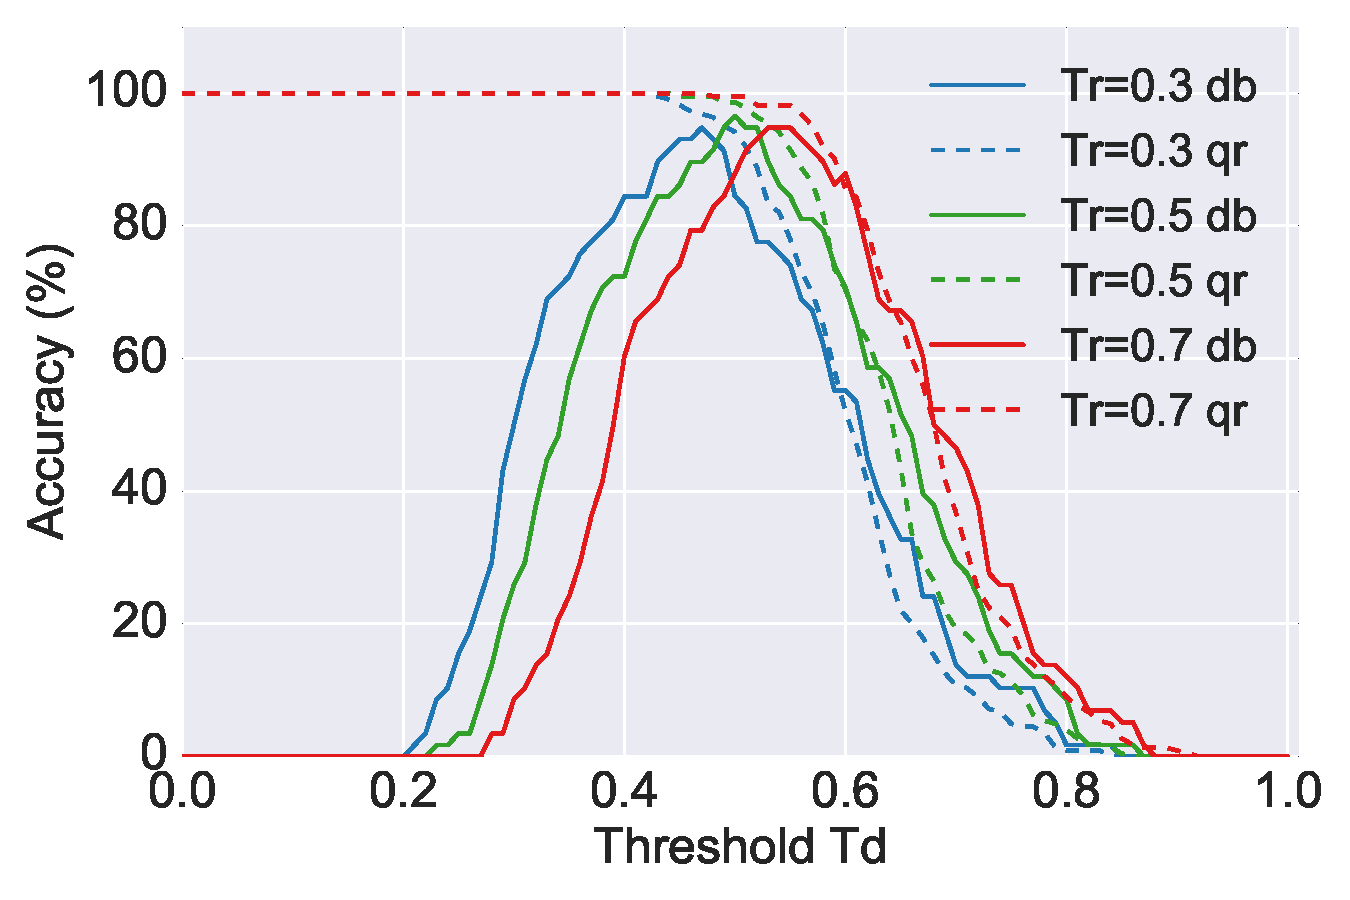
\includegraphics[width=\textwidth]{figure/ch4-accuracy-cosine.pdf}
        \caption{Cosine distance}
        \label{fig:ch4-acccosine}
      \end{subfigure}
    }
    \raisebox{-0.5\height}{
      \begin{subfigure}[b]{0.5\textwidth}
        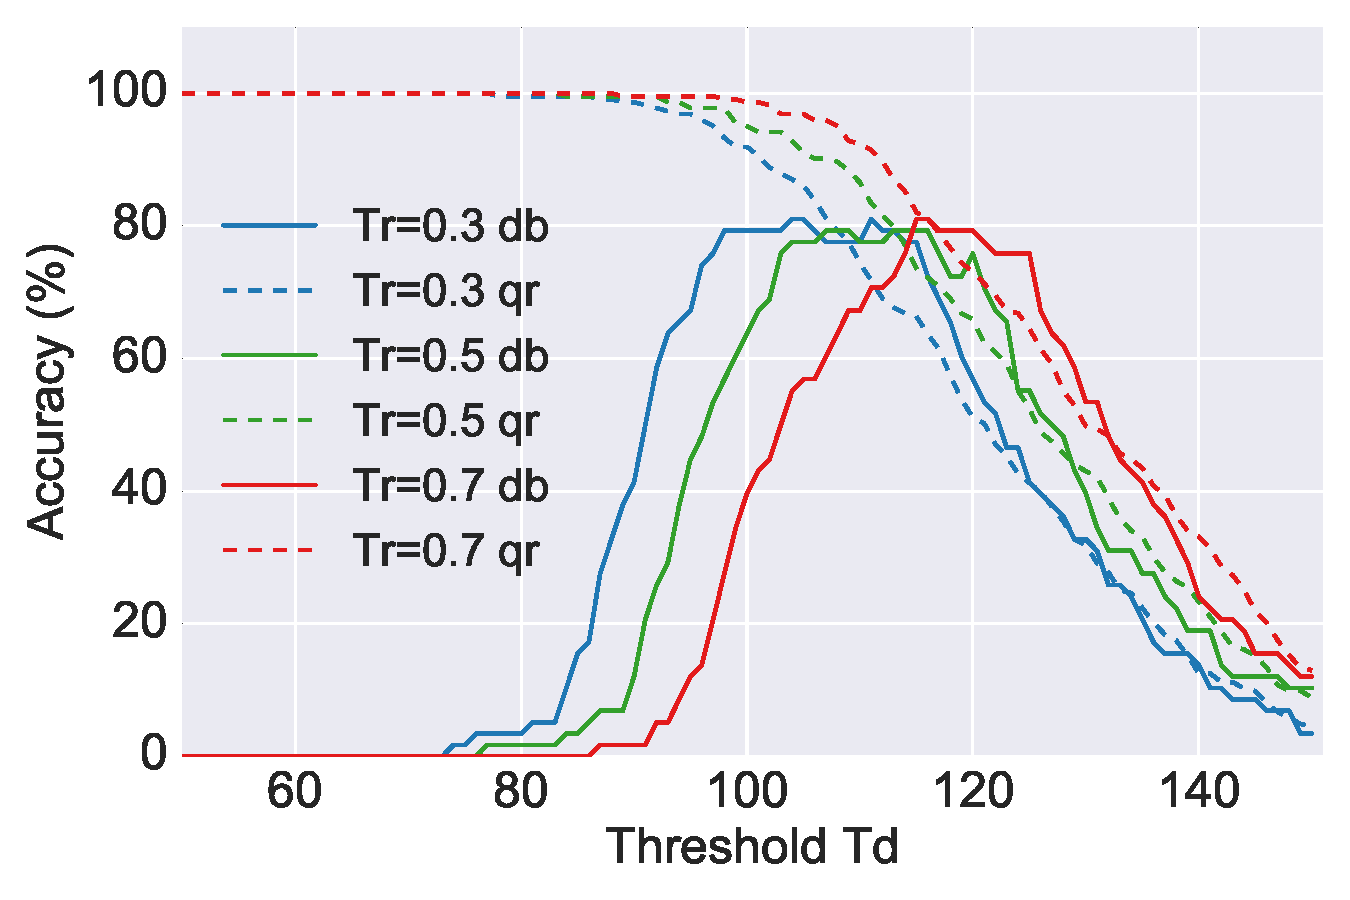
\includegraphics[width=\textwidth]{figure/ch4-accuracy-l2.pdf}
        \caption{Euclidean distance}
        \label{fig:ch4-accl2}
      \end{subfigure}
    }
  }
\caption{Face matching accuracy with different distance threshold $T_d$ and ratio threshold $T_r$.}
\label{fig:ch4-facematcheval}
\end{figure}

To evaluate face matching performance, we still use the user test set. Subjects who have more than $10$ features are regarded as the database group, the rest are the query group. Similar to face recognition accuracy, we break face matching accuracy into two parts: for persons belonging to the database group, we need to correctly match features only to the correct person; for persons not belonging to the database group, we should not match features to anyone. Figure~\ref{fig:ch4-facematcheval} shows the matching accuracy with Cosine distance and Euclidean distance respectively. The results show that Cosine distance can achieve better performance with near $100\%$ accuracy for both situations in which people belong to the database group or the query group. The preferable parameters would be distance threshold $T_d \approx 0.5$, and ratio threshold $T_r \approx 0.5$.

Overall, the face recognition and matching methods we employ with appropriate thresholds $T_p, T_d,$ and $T_r$ can effectively and efficiently recognize users and match faces in the images. Besides, only a small number of features are needed for training the face recognition model and for face matching algorithm.

\subsection{Gesture Recognition}

\begin{figure}[!htbp]
  \makebox[\textwidth]{
    \centering
    \raisebox{-0.5\height}{
      \begin{subfigure}[b]{0.4\textwidth}
        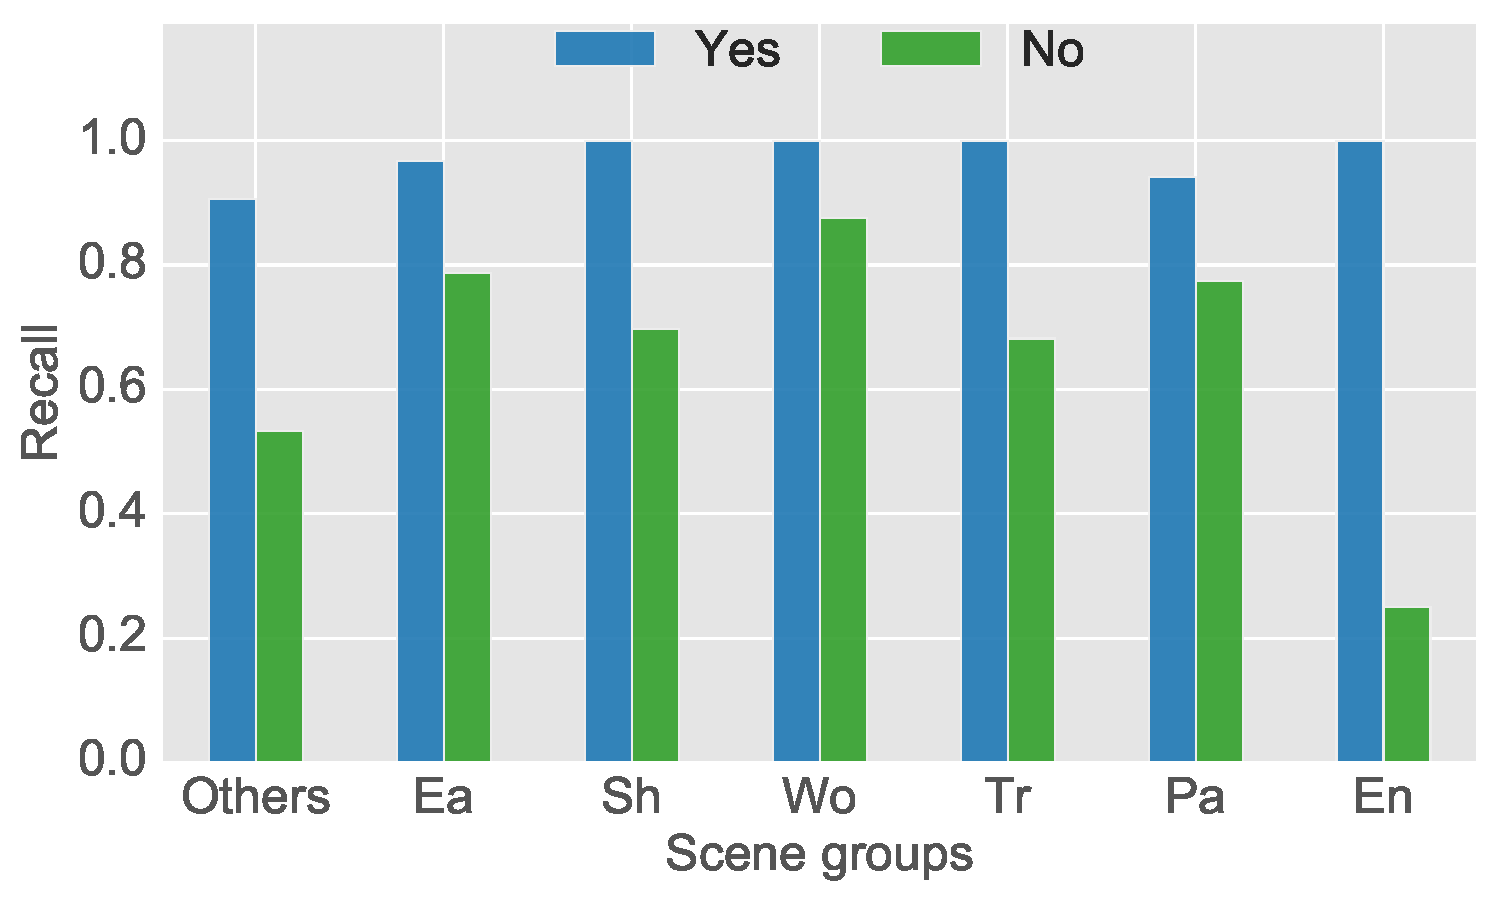
\includegraphics[width=\textwidth]{figure/ch4-hand-recall.pdf}
        \caption{Recall for different scenes}
        \label{fig:ch4-gestrecallscn}
      \end{subfigure}
    }
    \raisebox{-0.5\height}{
      \begin{subfigure}[b]{0.4\textwidth}
        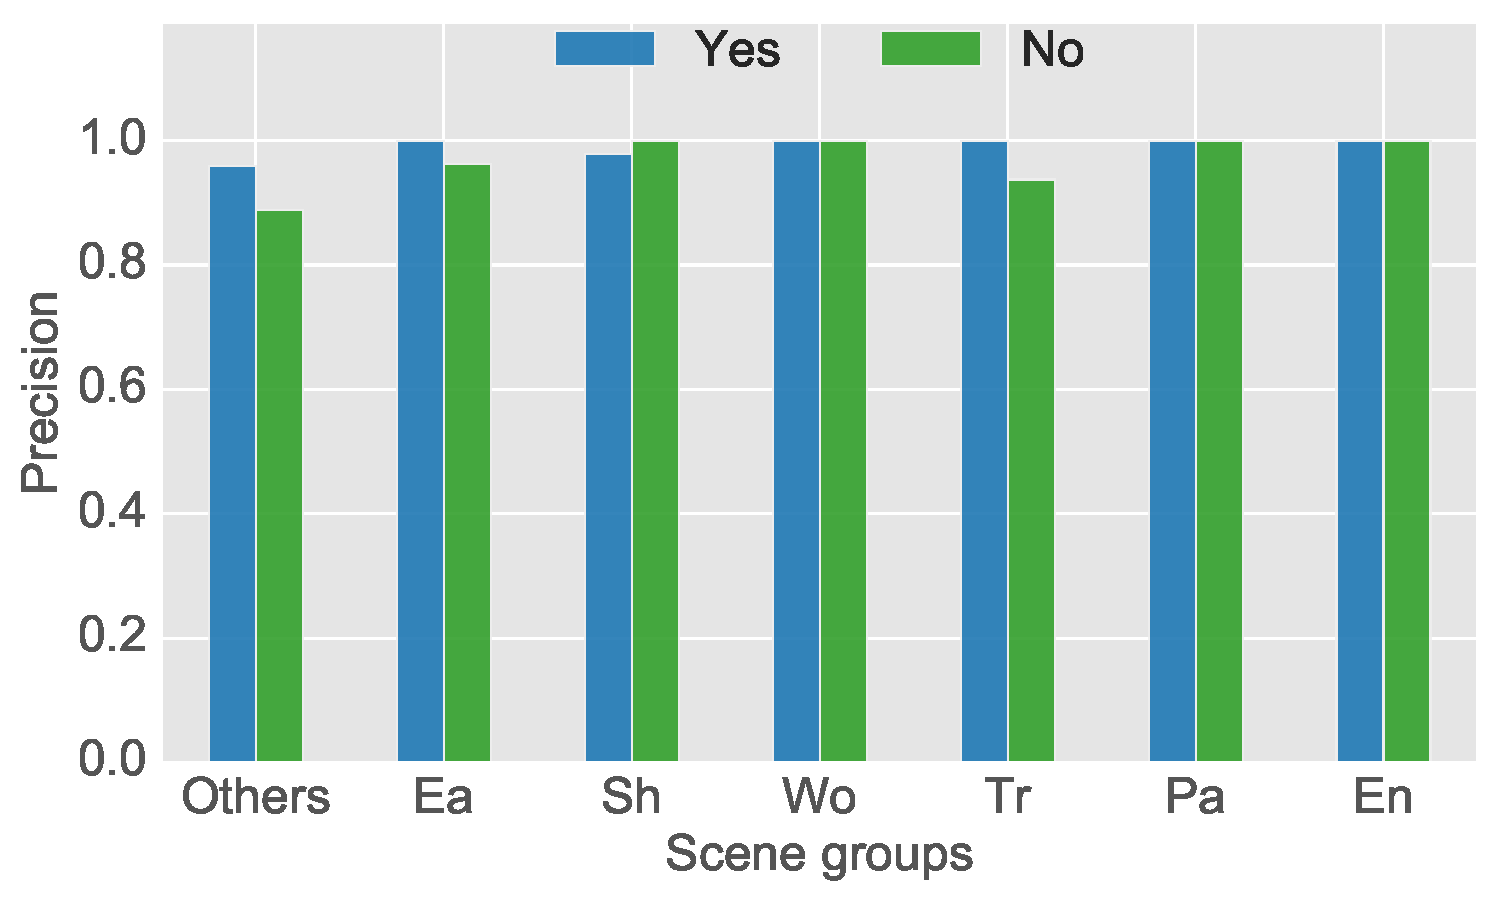
\includegraphics[width=\textwidth]{figure/ch4-hand-precision.pdf}
        \caption{Precision for different scenes}
        \label{fig:ch4-gestprecisionscn}
      \end{subfigure}
    }
    \raisebox{-0.5\height}{
      \begin{subfigure}[b]{0.4\textwidth}
        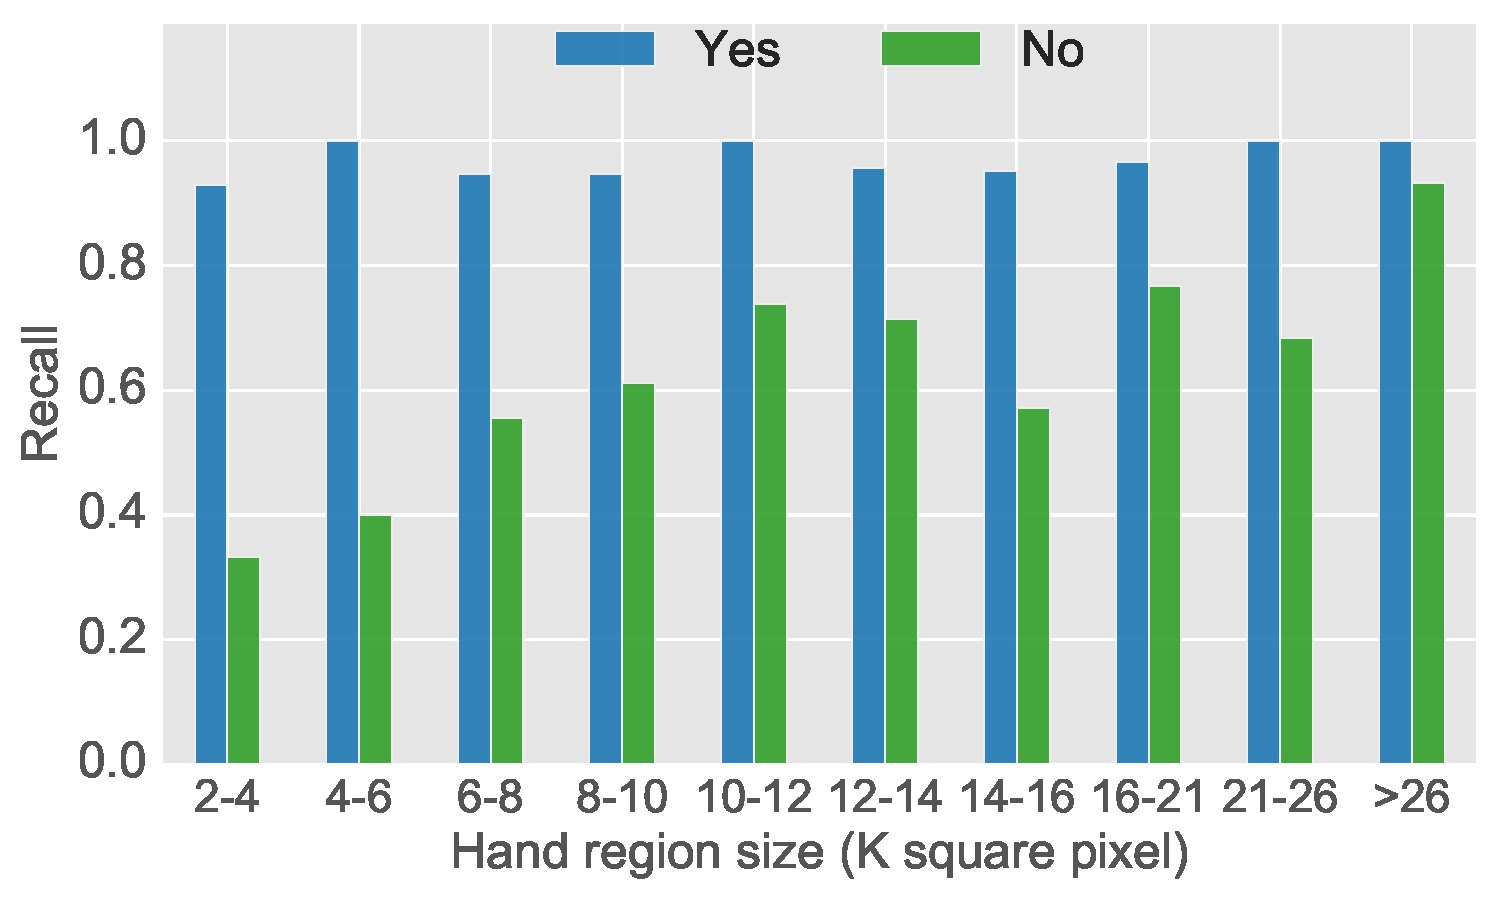
\includegraphics[width=\textwidth]{figure/ch4-hand-recall-size.pdf}
        \caption{Recall for different hand region sizes}
        \label{fig:ch4-gestrecallsize}
      \end{subfigure}
    }
  }
\caption{Hand gesture recognition results.}
\label{fig:ch4-gesteval}
\end{figure}

We asked our volunteers to take pictures for each other with different distances, angles, lighting conditions, and backgrounds. We manually annotated all images with hand regions and the scene group it belongs to. In total, we got $338$ hand gesture images with $208$ ``Yes'' gestures, $211$ ``No'' gestures, and $363$ natural hands. The images covers $6$ out of $9$ scene groups. For images do not belong to our summarized scene groups, we categorize them into group \textit{Others}.

Figure~\ref{fig:ch4-gestrecallscn} and Figure~\ref{fig:ch4-gestprecisionscn} show the recall and precision for ``Yes'' and ``No'' gestures under different scene groups. The recall and precision of ``Yes'' gesture, the precision of ``No'' gesture reach $1.0$ for most of the scene groups, while the recall of ``No'' gesture achieves $0.70$ on average. For \textit{Entertainment (En)}, the recall is low, resulting from dim illumination in most of the images we tested. In general, the performance of gesture recognition does not show any marked correlation with different scene groups. Therefore, we further investigated the recall in terms of gesture size, as low recall will greatly threatens user's privacy compared with precision.

Figure~\ref{fig:ch4-gestrecallsize} plots the recall of gestures with varying hand region sizes. Each image will be resized to about $800 \times 600$ square pixels, while keeping its aspect ratio. We classify them into $10$ size intervals as plotted along the \textit{x}--axis. The result shows ``Yes'' gestures can achieve more than $0.9$ recall for all sizes of hand region. On the other hand, recall of ``No'' gestures tends to rise with increasing hand region size in general. It indicates that the performance of ``No'' gesture recognition can be improved with more training data with smaller sizes.

In summary, the performance of gesture recognition demonstrates the feasibility of integrating gesture interaction in Cardea for flexible privacy preference modification. It performs extremely well for ``Yes'' gesture recognition, and there is room for improvement of ``No'' gesture recognition with more training samples.


\subsection{Overall Performance}

\begin{table}[tb]
\centering
\caption{Cardea's overall privacy protection performance.}
\label{tbl-overallperform}
\begin{tabular}{lr|lr}
\toprule
\textbf{Overall accuracy}   & $\mathbf{86.4\%}$ & Protection accuracy   & $80.4\%$  \\
                            &                   &  No protection accuracy& $91.0\%$ \\ \midrule
Face recognition accuracy   & $98.5\%$  & ``Yes'' gesture recall        & $97.9\%$  \\
scene classification recall & $77.7\%$  & ``No'' gesture recall     & $77.3\%$  \\ \bottomrule

\end{tabular}
\end{table}

After evaluating each vision task separately, we now present Cardea's overall privacy protection performance. Faces in the image taken using Cardea end up being protected (e.g., blurred) or remain unchanged, correctly or incorrectly, depending on protection decisions made based on both user's privacy profile and results from vision tasks. Therefore, we asked $5$ volunteers to register as Cardea users and set their privacy profiles. Now the face recognition model is trained using $1100$ face feature vectors from $55$ people, including $50$ people from LFW dataset. We take about $300$ images and get processed images. As we focus more on face recognition rather than face detection, we only keep images that faces have been successfully detected. In total we got $224$ images for evaluation.

Table~\ref{tbl-overallperform} shows the final privacy protection accuracy, as well as performance of each vision task. The protection accuracy shows $80.4\%$ faces that require protection are actually protected, and $91.0\%$ faces that do not ask for protection remain unchanged. Overall, $86.4\%$ faces are processed correctly, though the scene classification recall and ``No'' gesture recall do not reach $80\%$. The reason is that protection decision making process of Cardea sometimes can make up for mistakes happening in the early step. For example, if user's ``No'' gesture is not detected, his face can still be protected when the predict scene is selected in user's profile.

In summary, Cardea achieves over $85\%$ accuracy for users in the real world. Improvements of each vision part will directly benefit Cardea's overall performance in the future.


\subsection{Runtime and Energy Consumption}
We validate the client side implementations on Samsung Galaxy Note 4\footnote{\url{http://www.gsmarena.com/samsung_galaxy_note_4-6434.php}}, with 4$\times$2.7 GHz Krait 450 CPU, Qualcomm Snapdragon 805 Chipset, 3GB RAM, and 16 MP, f/2.2 Camera. The server side is configured with Intel i7--5820K CPU, 16GB RAM, GeForce 980Ti Graphic Card (6GB RAM). The client and server communicate via a TCP over Wi--Fi connection.

\begin{figure}[tb]
\centering
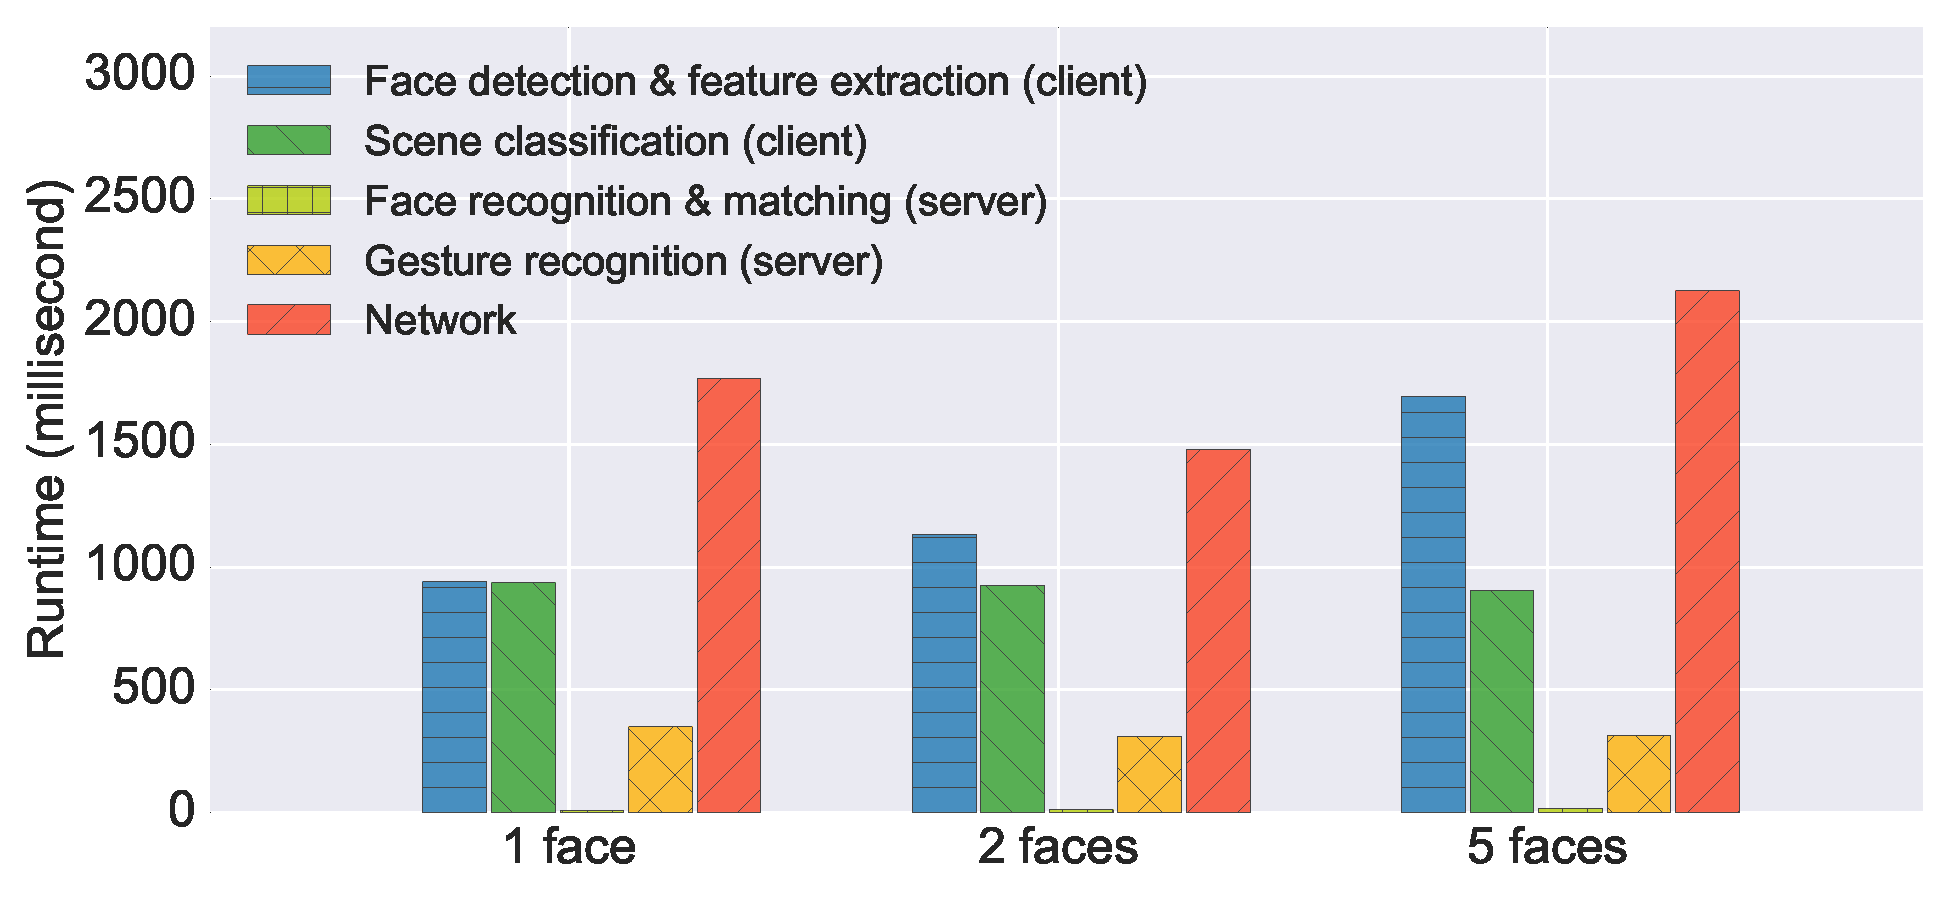
\includegraphics[width=0.8\textwidth]{figure/ch4-runtime.pdf}
\caption{Task level runtime of Cardea.}
\label{fig:ch4-runtime}
\end{figure}

Figure~\ref{fig:ch4-runtime} plots the time taken for Cardea to complete different vision tasks. We take images with $1$ face, $2$ faces, and $5$ faces, in the size of $1920 \times 1080$. The images will be compressed in JPEG format. On average, the data sent is about $950$ KB. Note that some vision tasks will not be triggered in some situations according to the decision workflow shown in Fig~\ref{fig:ch4-decisiontree}. For example, if no user is recognized in the image, all other tasks will not start. For the purpose of measurement, we still activate all tasks to illustrate the runtime difference of images captured with varying number of faces.

Among all vision tasks, face processing (i.e., face detection and feature extraction) and scene classification are performed on the smartphone. The face processing takes about $900$ milliseconds for 1 face, and increases about $200$ milliseconds per additional face. Therefore, it reaches about $1100$ and $1700$ milliseconds for $2$ faces and $5$ faces respectively. This is the most fundamental step that runs on the smartphone locally due to privacy considerations. Owing to the real--time OpenCV face detection implementation and lightened CNN feature extraction model, it takes less then $1/3$ overall runtime. The scene classification takes around $900$ milliseconds per image, as it only performs once, independent of number of people in the image. The face recognition and matching tasks on the server side take less than $30$ milliseconds for five people. Though the time grows with increasing number of people, compared with other tasks they barely affect the overall runtime. The gesture recognition also runs on the server, and it takes about $330$ milliseconds. Similar to scene recognition, it performs on the whole image once regardless the number of faces. According to the measurement, we find the network transmission accounts for a majority of the overall runtime due to the unstable network environment.

In general, photographers using Cardea to take pictures can get one processed image within $5$ seconds in the most heavy case (i.e., there is registered user who enables gestures, and scene classification will be triggered on the smartphone). Compared with existing image capture platforms that also provide privacy protection such as I-pic \cite{aditya2016pic}, Cardea offers more efficient image processing functionality.

\begin{table}[tb]
\centering
\caption{Energy consumption of Cardea with different number of faces.}
\label{tbl-energy}
\begin{tabular}{lrrr}
\toprule
            & Face recognition      & Whole process (uAh)   & \# of images \\ \midrule
1 face      & $217.2$ (std $3.4$)   & $1134.5$ (std $45.9$) & $\sim 2800$       \\
2 faces     & $344.1$ (std $13.1$)  & $1276.7$ (std $113.8$)    & $\sim 2500$       \\
5 faces     & $692.6$ (std $36.5$)  & $1641.1$ (std $66.0$) & $\sim 2000$       \\ \bottomrule
\end{tabular}
\end{table}

Next, we measure the energy consumption of taking pictures with Cardea on Galaxy Note 4 phone using the Monsoon Power Monitor \cite{links:powermonitor}. The images are also taken in size of $1920 \times 1080$ square pixels. The first two columns of Table~\ref{tbl-energy} show the energy consumption for the face processing part only, and for the whole process (i.e., from taking a picture to getting the processed image) with 1 face, 2 faces, and 5 faces respectively. The screen stays on during the whole process, therefore a large portion of the energy consumption is due to the always--on screen. Moreover, we can observe that face processing energy is linear to face numbers. All the other parts including scene classification, sending and receiving data are independent of the number of faces in the image, which is consistent with runtime measurements.

Using energy measurements, we also show Cardea's capacity on Galaxy Note 4 in the last column of Table~\ref{tbl-energy}. This device has a $3220$ mAh battery, therefore can capture about $2000$ high quality images with $5$ faces using Cardea.



\newpage
